% !TEX program = xelatex
\documentclass[11pt,a4paper]{ctexart}
% Shared preamble for the assignment reports. Use with:
%   \documentclass[11pt,a4paper]{ctexart}  (XeLaTeX)
%   % Shared preamble for the assignment reports. Use with:
%   \documentclass[11pt,a4paper]{ctexart}  (XeLaTeX)
%   % Shared preamble for the assignment reports. Use with:
%   \documentclass[11pt,a4paper]{ctexart}  (XeLaTeX)
%   \input{../common/preamble.tex}
\usepackage[margin=2.3cm]{geometry}
\setmainfont{texgyretermes}[Extension=.otf,UprightFont=*-regular,BoldFont=*-bold,ItalicFont=*-italic,BoldItalicFont=*-bolditalic]
\setsansfont{texgyreheros}[Extension=.otf,UprightFont=*-regular,BoldFont=*-bold,ItalicFont=*-italic,BoldItalicFont=*-bolditalic]
\setmonofont{texgyrecursor}[Extension=.otf,UprightFont=*-regular,BoldFont=*-bold,ItalicFont=*-italic,BoldItalicFont=*-bolditalic]
\usepackage{amsmath,amssymb,mathtools,bm}
\usepackage{graphicx}
\usepackage{booktabs,multirow,makecell,array,tabularx}
\usepackage[table]{xcolor}
\usepackage[most]{tcolorbox}
\usepackage{enumitem}
\usepackage{listings}
\usepackage{subcaption}
\usepackage{siunitx}
\usepackage[hidelinks]{hyperref}
\usepackage[nameinlink,noabbrev]{cleveref}
\usepackage{float}

\setlength{\emergencystretch}{3em}
\linespread{1.15}
\setlist{leftmargin=*,itemsep=2pt,topsep=3pt}
\graphicspath{{figures/}}

\crefname{figure}{图}{图}
\crefname{table}{表}{表}
\crefname{section}{第}{第}
\creflabelformat{section}{#2#1#3 节}
\crefname{equation}{式}{式}
\crefformat{equation}{式~(#2#1#3)}

\lstset{basicstyle=\ttfamily\footnotesize,columns=fullflexible,breaklines=true,frame=single,
  framerule=0.3pt,rulecolor=\color{black!40},backgroundcolor=\color{black!3},
  keywordstyle=\color{blue!60!black}\bfseries,commentstyle=\color{green!40!black},
  numbers=left,numberstyle=\tiny\color{black!50},xleftmargin=1.5em}

% Interview boxes: question, model answer, common wrong answer.
\newtcolorbox{iqbox}[1]{enhanced,breakable,colback=blue!3,colframe=blue!45!black,boxrule=0.5pt,arc=1.5pt,
  left=4pt,right=4pt,top=3pt,bottom=3pt,fonttitle=\bfseries\small,title={面试追问：#1}}
\newtcolorbox{findingbox}[1][]{enhanced,breakable,colback=green!3,colframe=green!40!black,boxrule=0.5pt,arc=1.5pt,
  left=4pt,right=4pt,top=3pt,bottom=3pt,fonttitle=\bfseries\small,title={结论#1}}
\newtcolorbox{caveatbox}{enhanced,breakable,colback=orange!4,colframe=orange!60!black,boxrule=0.5pt,arc=1.5pt,
  left=4pt,right=4pt,top=3pt,bottom=3pt,fonttitle=\bfseries\small,title={不能推出的结论}}

\newcommand{\authorline}{ShaneLiu04\thanks{GitHub: \url{https://github.com/ShaneLiu04}。代码与原始指标：\url{https://gitee.com/liu-xingyan04/mlsys-infra}。本文基于公开课程材料独立完成，与课程团队无隶属关系。}}

\usepackage[margin=2.3cm]{geometry}
\setmainfont{texgyretermes}[Extension=.otf,UprightFont=*-regular,BoldFont=*-bold,ItalicFont=*-italic,BoldItalicFont=*-bolditalic]
\setsansfont{texgyreheros}[Extension=.otf,UprightFont=*-regular,BoldFont=*-bold,ItalicFont=*-italic,BoldItalicFont=*-bolditalic]
\setmonofont{texgyrecursor}[Extension=.otf,UprightFont=*-regular,BoldFont=*-bold,ItalicFont=*-italic,BoldItalicFont=*-bolditalic]
\usepackage{amsmath,amssymb,mathtools,bm}
\usepackage{graphicx}
\usepackage{booktabs,multirow,makecell,array,tabularx}
\usepackage[table]{xcolor}
\usepackage[most]{tcolorbox}
\usepackage{enumitem}
\usepackage{listings}
\usepackage{subcaption}
\usepackage{siunitx}
\usepackage[hidelinks]{hyperref}
\usepackage[nameinlink,noabbrev]{cleveref}
\usepackage{float}

\setlength{\emergencystretch}{3em}
\linespread{1.15}
\setlist{leftmargin=*,itemsep=2pt,topsep=3pt}
\graphicspath{{figures/}}

\crefname{figure}{图}{图}
\crefname{table}{表}{表}
\crefname{section}{第}{第}
\creflabelformat{section}{#2#1#3 节}
\crefname{equation}{式}{式}
\crefformat{equation}{式~(#2#1#3)}

\lstset{basicstyle=\ttfamily\footnotesize,columns=fullflexible,breaklines=true,frame=single,
  framerule=0.3pt,rulecolor=\color{black!40},backgroundcolor=\color{black!3},
  keywordstyle=\color{blue!60!black}\bfseries,commentstyle=\color{green!40!black},
  numbers=left,numberstyle=\tiny\color{black!50},xleftmargin=1.5em}

% Interview boxes: question, model answer, common wrong answer.
\newtcolorbox{iqbox}[1]{enhanced,breakable,colback=blue!3,colframe=blue!45!black,boxrule=0.5pt,arc=1.5pt,
  left=4pt,right=4pt,top=3pt,bottom=3pt,fonttitle=\bfseries\small,title={面试追问：#1}}
\newtcolorbox{findingbox}[1][]{enhanced,breakable,colback=green!3,colframe=green!40!black,boxrule=0.5pt,arc=1.5pt,
  left=4pt,right=4pt,top=3pt,bottom=3pt,fonttitle=\bfseries\small,title={结论#1}}
\newtcolorbox{caveatbox}{enhanced,breakable,colback=orange!4,colframe=orange!60!black,boxrule=0.5pt,arc=1.5pt,
  left=4pt,right=4pt,top=3pt,bottom=3pt,fonttitle=\bfseries\small,title={不能推出的结论}}

\newcommand{\authorline}{ShaneLiu04\thanks{GitHub: \url{https://github.com/ShaneLiu04}。代码与原始指标：\url{https://gitee.com/liu-xingyan04/mlsys-infra}。本文基于公开课程材料独立完成，与课程团队无隶属关系。}}

\usepackage[margin=2.3cm]{geometry}
\setmainfont{texgyretermes}[Extension=.otf,UprightFont=*-regular,BoldFont=*-bold,ItalicFont=*-italic,BoldItalicFont=*-bolditalic]
\setsansfont{texgyreheros}[Extension=.otf,UprightFont=*-regular,BoldFont=*-bold,ItalicFont=*-italic,BoldItalicFont=*-bolditalic]
\setmonofont{texgyrecursor}[Extension=.otf,UprightFont=*-regular,BoldFont=*-bold,ItalicFont=*-italic,BoldItalicFont=*-bolditalic]
\usepackage{amsmath,amssymb,mathtools,bm}
\usepackage{graphicx}
\usepackage{booktabs,multirow,makecell,array,tabularx}
\usepackage[table]{xcolor}
\usepackage[most]{tcolorbox}
\usepackage{enumitem}
\usepackage{listings}
\usepackage{subcaption}
\usepackage{siunitx}
\usepackage[hidelinks]{hyperref}
\usepackage[nameinlink,noabbrev]{cleveref}
\usepackage{float}

\setlength{\emergencystretch}{3em}
\linespread{1.15}
\setlist{leftmargin=*,itemsep=2pt,topsep=3pt}
\graphicspath{{figures/}}

\crefname{figure}{图}{图}
\crefname{table}{表}{表}
\crefname{section}{第}{第}
\creflabelformat{section}{#2#1#3 节}
\crefname{equation}{式}{式}
\crefformat{equation}{式~(#2#1#3)}

\lstset{basicstyle=\ttfamily\footnotesize,columns=fullflexible,breaklines=true,frame=single,
  framerule=0.3pt,rulecolor=\color{black!40},backgroundcolor=\color{black!3},
  keywordstyle=\color{blue!60!black}\bfseries,commentstyle=\color{green!40!black},
  numbers=left,numberstyle=\tiny\color{black!50},xleftmargin=1.5em}

% Interview boxes: question, model answer, common wrong answer.
\newtcolorbox{iqbox}[1]{enhanced,breakable,colback=blue!3,colframe=blue!45!black,boxrule=0.5pt,arc=1.5pt,
  left=4pt,right=4pt,top=3pt,bottom=3pt,fonttitle=\bfseries\small,title={面试追问：#1}}
\newtcolorbox{findingbox}[1][]{enhanced,breakable,colback=green!3,colframe=green!40!black,boxrule=0.5pt,arc=1.5pt,
  left=4pt,right=4pt,top=3pt,bottom=3pt,fonttitle=\bfseries\small,title={结论#1}}
\newtcolorbox{caveatbox}{enhanced,breakable,colback=orange!4,colframe=orange!60!black,boxrule=0.5pt,arc=1.5pt,
  left=4pt,right=4pt,top=3pt,bottom=3pt,fonttitle=\bfseries\small,title={不能推出的结论}}

\newcommand{\authorline}{ShaneLiu04\thanks{GitHub: \url{https://github.com/ShaneLiu04}。代码与原始指标：\url{https://gitee.com/liu-xingyan04/mlsys-infra}。本文基于公开课程材料独立完成，与课程团队无隶属关系。}}

\graphicspath{{../../solutions/cs149/asst1-cpu-parallel/artifacts/figures/}}

\title{CS149 Assignment 1 实验报告：\\多核、SIMD、带宽与 GPU 对照}
\author{\authorline}
\date{2026 年 10 月}

\begin{document}
\maketitle

\begin{abstract}
本文完成 Stanford CS149（Fall 2024）Assignment 1 ``Analyzing Parallel Program Performance on a Quad-Core CPU''
的全部六个 program，并把同样的三个问题——负载均衡、SIMD 发散、内存带宽——搬到 GPU 上做对照。
实现全部用 C++17：\texttt{std::thread} 版 Mandelbrot、自写的 CS149 fake vector intrinsics、
用 AVX2/AVX-512 intrinsics 手写的 ISPC gang（无 ISPC 编译器）、Newton 法 sqrt、带 non-temporal store 的
saxpy 以及 K-means 的 profiling 与三级优化；GPU 部分用 CUDA 在 RTX 5090 上实现。
所有 SIMD、多线程和 GPU 结果都与标量参考\textbf{逐位相等}（编译时关闭 FMA 合并），
计时取 3 轮独立实验的中位数并给出最小--最大区间。
主要结论：(1) 连续块静态划分在 view~1 上 12 线程只有 5.89 倍，动态分块达到 11.1 倍；
(2) Mandelbrot 内核受依赖链延迟限制，一个物理核上的两个 SMT 线程几乎等于两个核，
单线程交错两组向量（ILP）把 AVX-512 加速从 11.2 倍提到 18.3 倍，超过 16 lane 的宽度；
(3) Newton sqrt 在``每 W 个元素 1 个慢''的输入下，AVX2 比标量还慢（0.72 倍），AVX-512 在三种发散程度不同的输入上耗时完全相同；
(4) saxpy 单线程只能拿到 23~GB/s 的 DRAM 带宽，12 线程 173~GB/s，streaming store 省掉 write-allocate 后再高 3\%--33\%，
跨 socket 访问降 30\%；(5) K-means 只并行化 \texttt{computeAssignments} 时受 Amdahl 定律限制在 2.1 倍，
三个阶段全部并行并做循环交换和向量化后达到 11.7 倍；(6) 同一 Mandelbrot 在 RTX 5090 上比 12 核 AVX-512 双向量交错版再快 60--100 倍，
但 saxpy 只要数据需要跨 PCIe，GPU 端到端吞吐（52~GB/s）就低于 CPU。
每一节最后给出面试问法与常见错答。
\end{abstract}

\tableofcontents
\newpage

%====================================================================
\section{作业要求与本文实现}
\label{sec:intro}

CS149~\cite{cs149} Assignment 1 的目标是让学生在一台四核 CPU 上亲手测出并行程序的三类瓶颈。表~\ref{tab:map} 给出官方六个 program
与本文实现的对应关系。官方 starter 依赖 ISPC~\cite{ispc} 编译器与 C++，本文在 Windows 本机（MinGW g++ 13）和 Linux 服务器（g++ 11）上
用同一份代码编译运行；ISPC 的 gang 与 task 用 AVX2/AVX-512 intrinsics~\cite{intel} 和一个原子计数器分发的线程池替代。

\begin{table}[H]
\centering
\caption{官方 program 与本文实现}
\label{tab:map}
\small
\begin{tabularx}{\linewidth}{>{\raggedright}p{2.6cm}>{\raggedright}X>{\raggedright\arraybackslash}X}
\toprule
官方 program & 官方要回答的问题 & 本文实现（\texttt{cpp/}） \\
\midrule
prog1 Mandelbrot threads & 线程数与加速比；为什么连续块划分不线性；如何划分到 7--8 倍 & 连续块、隔行、动态分块三种调度，1--24 线程，SMT~\cite{smt} 与 NUMA 布局，每线程计时 \\
prog2 vector intrinsics & 用 fake intrinsics 写 \texttt{clampedExp} 与 \texttt{arraySum}，统计 lane 利用率随宽度的变化 & 自写 \texttt{cs149intrin.h}（同名 API 与 logger），W=2/4/8/16，5 种指数分布 \\
prog3 ISPC Mandelbrot & gang 加速比为什么不到 8；task 数量的选择 & AVX2 8 lane、AVX-512 16 lane、AVX-512 双向量交错；task 数 1--1200 扫描 \\
prog4 sqrt & 构造让 ISPC 加速最好和最差的输入 & 标量、AVX2、AVX-512、SIMD+线程；random / all\_slow / all\_one / one\_slow\_8 / one\_slow\_16 \\
prog5 saxpy & 为什么多核加速有限；写回带来的额外流量 & 标量、SIMD、streaming store、纯读四个内核，工作集 12~KB--1.6~GB，NUMA \\
prog6 K-means~\cite{lloyd} & 用计时找瓶颈并优化 & 官方结构的 baseline 与 v1/v2/v3 三级优化，分阶段计时 \\
\bottomrule
\end{tabularx}
\end{table}

此外有两部分是作业之外的补充：第~\ref{sec:gpu}~节把 prog3/4/5/6 的核心内核写成 CUDA，在 RTX 5090 上回答``同一个问题在 SIMT~\cite{tesla} 上
答案是否一样''；第~\ref{sec:python}~节简要回顾仓库中原有的 Python 版本，说明为什么解释器版本的数字不能用来回答作业问题。

%====================================================================
\section{实验平台与方法}
\label{sec:setup}

\subsection{硬件与软件}

\begin{table}[H]
\centering
\caption{实验平台}
\label{tab:platform}
\small
\begin{tabularx}{\linewidth}{lXX}
\toprule
 & 服务器（主平台） & 本机（四核对照） \\
\midrule
CPU & 2 $\times$ Intel Xeon Gold 6459C（Sapphire Rapids），每路 32 核，SMT 2 & Intel Ice Lake 服务器核（虚拟机），4 核 8 线程 \\
缓存 & 每核 L1d 48~KB、L2 2~MB；每路 L3 60~MB & 每核 L1d 48~KB、L2 1.25~MB；L3 57~MB \\
可用 CPU & cgroup 配额 16 个 CPU；本文固定绑在 socket~0 的 12 个空闲物理核上 & 4 物理核，SMT 兄弟为 $(2k, 2k{+}1)$ \\
内存 & 754~GB，2 个 NUMA 节点 & 32~GB \\
ISA & AVX2、AVX-512（含 BF16/FP16）、AMX & AVX2、AVX-512 \\
GPU & NVIDIA RTX 5090（sm\_120，170 SM，32~GB GDDR7，512 bit，96~MB L2） & 无 \\
编译器 & g++ 11.4，CUDA 12.8 & MinGW-w64 g++ 13.2 \\
\bottomrule
\end{tabularx}
\end{table}

服务器是多租户宿主机：容器能看到 128 个逻辑 CPU，但 cgroup 只给 16 个 CPU 的时间配额，而且其他租户会占满个别核。
开始实验前用 \texttt{/proc/stat} 采样 3 秒，发现 CPU~15、20 被其他租户占到 99\%，于是固定使用 socket~0 上的
\{0,1,2,3,4,6,10,11,14,16,19,23\} 这 12 个物理核；SMT 实验使用它们的兄弟 $c{+}64$，NUMA 实验使用 socket~1 的 12 个空闲核。
拓扑由 \texttt{lscpu -e}（Linux）和 \texttt{GetLogicalProcessorInformationEx}（Windows，本文的 \texttt{topology.exe}）确认。

\subsection{正确性}

所有程序用 \texttt{-O3 -march=native -ffp-contract=off} 编译。\texttt{-ffp-contract=off} 禁止编译器把 $a\cdot b+c$ 合并成 FMA，
这样手写的 SIMD 内核只要逐操作照搬标量代码的运算顺序（例如先算 \texttt{2*zr} 再乘 \texttt{zi}），结果就与标量版本逐位相等。
比较 $|z|^2>4$ 时用 \texttt{\_CMP\_NGT\_UQ}（``不大于''，NaN 时为真）而不是 \texttt{\_CMP\_LE\_OQ}，与标量 \texttt{!(x>4)} 的 NaN 语义一致。
每个程序在每次测量后检查结果，任何不一致都会让进程以非零码退出；\texttt{tests/test\_cpp.py} 用小规模输入跑全部六个 program。
GPU 版用 \texttt{nvcc -fmad=false} 编译，host 端参考使用相同的运算顺序，Mandelbrot 与 sqrt 同样逐位相等（mismatch = 0）。

\subsection{计时}

每个配置取 $N$ 次运行的最小值（prog1/3 为 7 次，prog4 为 3 次），与官方 starter 的做法相同；整个实验在服务器上独立重复 3 轮，
文中数字为 3 轮的中位数，图中误差棒为最小--最大值。prog5 用常驻自旋线程池，每个尺寸至少运行 0.2~s。
服务器的单线程 turbo 频率高于全核频率，这会让多线程加速比天然低于线性，第~\ref{sec:prog1}~节会看到这一点。

%====================================================================
\section{Program 1：线程与负载均衡}
\label{sec:prog1}

\subsection{工作量的空间分布}

\cref{fig:views} 左侧是两个视图的迭代数，右侧是每行的总工作量（迭代数 $+1$，最后一次判断也算）。view~1 的中间几行穿过
Mandelbrot 集主体，每个像素都跑满 256 次；边缘行几乎立刻逃逸。把 1200 行切成 $P$ 个连续块时，最重的块决定完成时间，
静态划分的加速比上限为
\begin{equation}
S_{\text{block}} \le \frac{\sum_r w_r}{\max_{k}\sum_{r\in B_k} w_r} = \frac{P}{\max_k W_k / \bar W}.
\label{eq:blockbound}
\end{equation}
图中标注了 $P=4$ 与 $P=12$ 时的 $\max/\text{mean}$：view~1 分别为 1.61 和 2.00，即连续块划分在 12 线程时上限只有 6 倍；
view~2 是 1.49 和 1.97。

\begin{figure}[H]
\centering
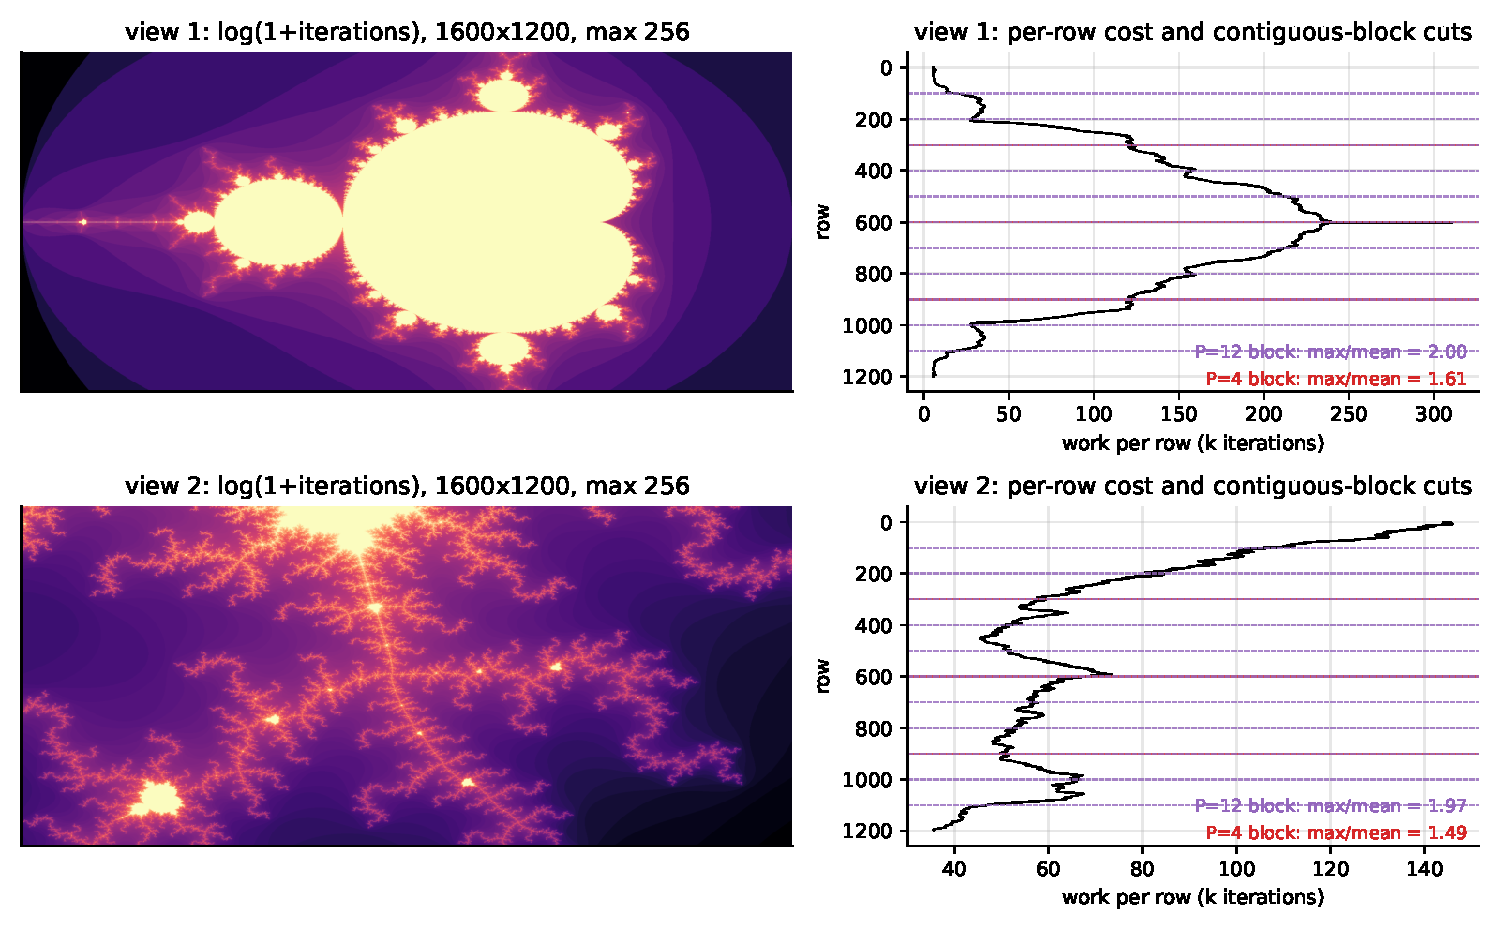
\includegraphics[width=\linewidth]{cpp_mandel_views.pdf}
\caption{左：两个视图的 $\log(1+\text{迭代数})$；右：每行工作量与 $P=4$（实线）、$P=12$（虚线）的连续块切分线。}
\label{fig:views}
\end{figure}

\subsection{三种调度的加速比}

\cref{fig:speedup} 是加速比随线程数的变化。三种调度的差别正好对应式~\eqref{eq:blockbound}：

\begin{itemize}
\item \textbf{连续块（block）}：view~1 在 3 线程时只有 1.64 倍，比 2 线程（1.99）还低，因为 3 等分让中间那块独揽整个集合主体；
12 线程 5.89 倍，接近式~\eqref{eq:blockbound} 给出的 6 倍上限。
\item \textbf{隔行（interleaved）}：线程 $t$ 取第 $t, t{+}P, \dots$ 行，把相邻行的相关性打散，按工作量几乎完全均衡；
但它仍是静态划分，任何一个核被其他租户抢占，所有线程都要等它。
\item \textbf{动态（dynamic，每次取 4 行）}：线程从原子计数器领任务，既均衡工作量，也自动绕开慢核。view~1 在 8 线程达到 7.74 倍，12 线程 11.1 倍。
\end{itemize}

\begin{figure}[H]
\centering
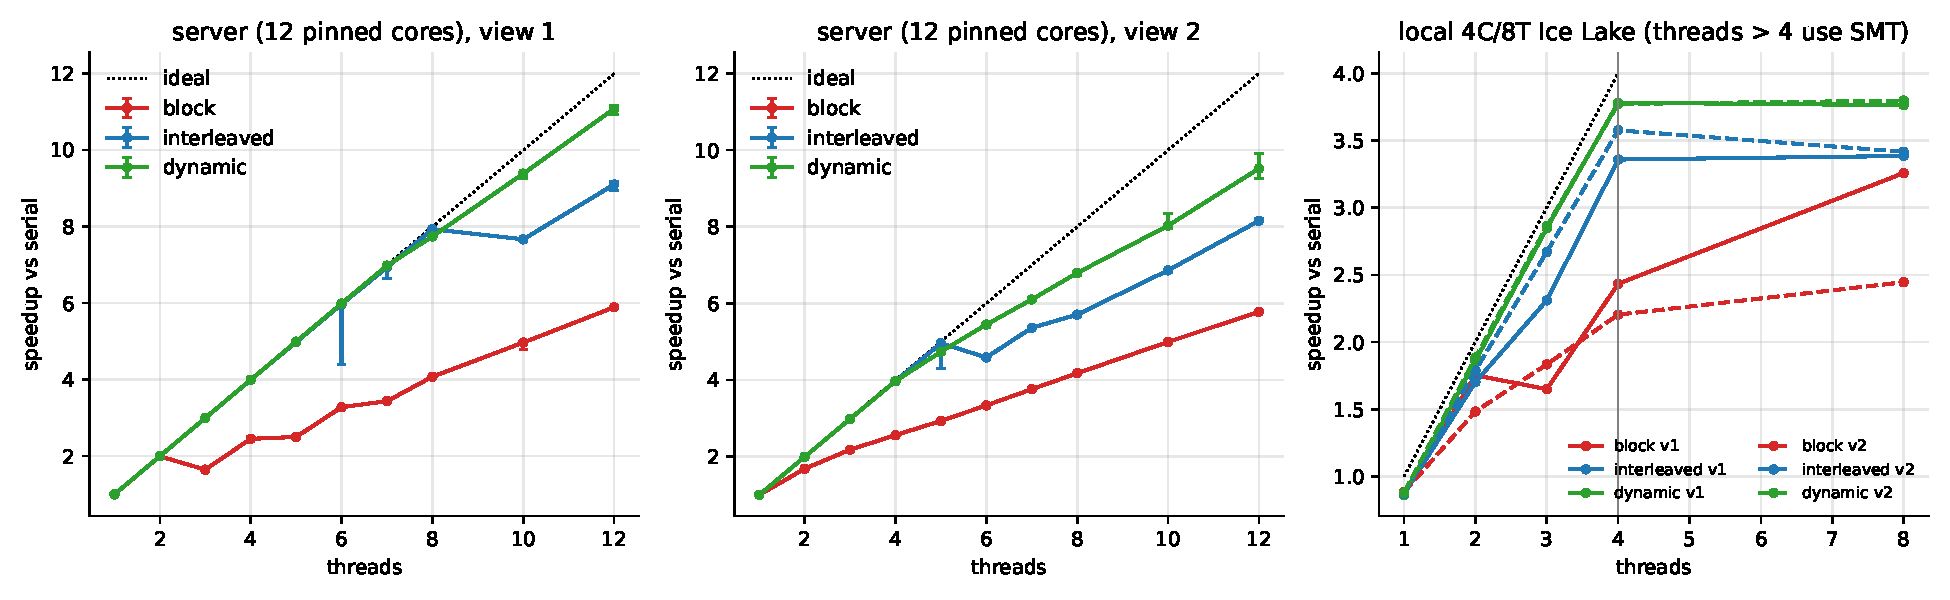
\includegraphics[width=\linewidth]{cpp_prog1_speedup.pdf}
\caption{prog1 加速比。左、中：服务器 12 个绑定物理核，3 轮中位数与最小--最大区间；右：本机四核（4 线程以上使用 SMT）。}
\label{fig:speedup}
\end{figure}

\cref{fig:threadtime} 展示 8 线程时每个线程的计算时间。连续块划分下 0 号和 7 号线程几乎无事可做，3、4 号线程决定墙钟时间；
隔行和动态划分下 8 个线程的时间几乎一样，墙钟时间约为连续块的一半。这张图就是面试中``为什么加线程不线性''最直接的证据：
墙钟时间等于最慢线程的时间，而不是平均时间。

\begin{figure}[H]
\centering
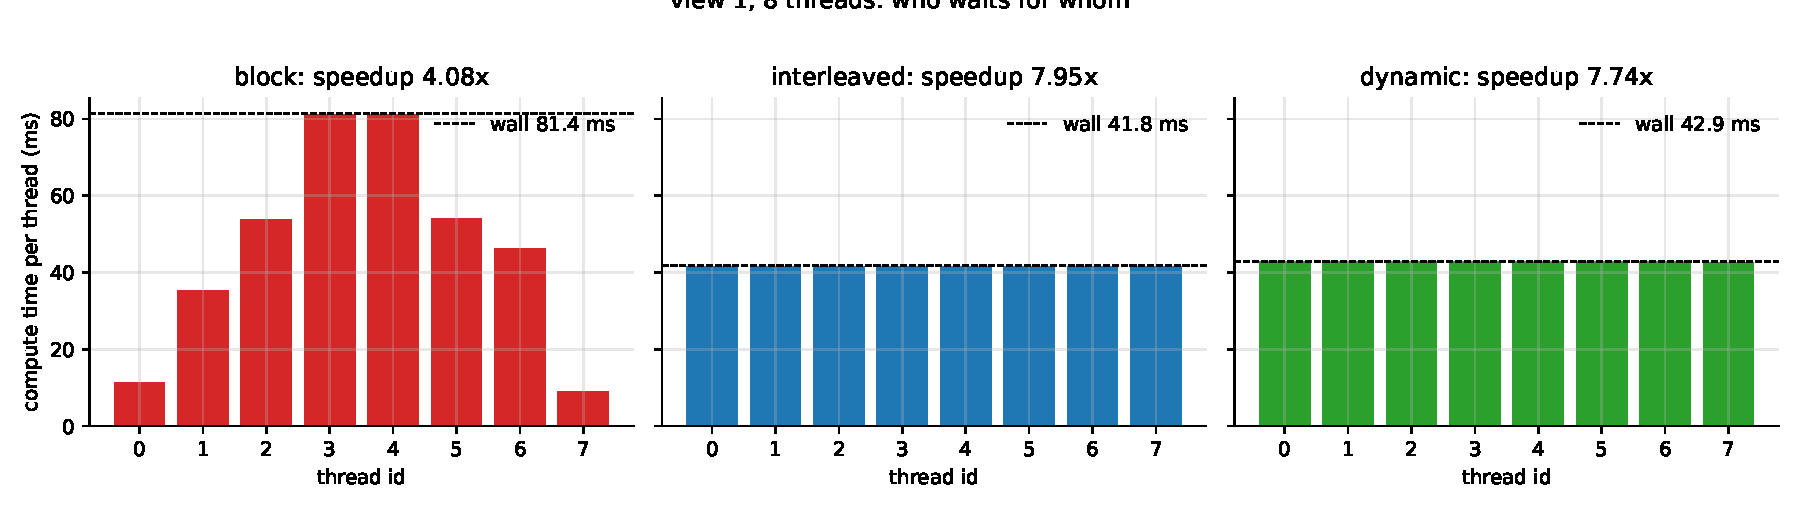
\includegraphics[width=\linewidth]{cpp_prog1_thread_time.pdf}
\caption{view~1、8 线程时每个线程的计算时间，虚线为墙钟时间。}
\label{fig:threadtime}
\end{figure}

\subsection{动态分块的粒度}

\cref{fig:chunk} 扫描每次领取的行数。chunk 为 1--16 行时加速比基本持平（12 线程 view~1 为 9.2--9.5 倍），32 行开始下降，
chunk 增大到 100 行（每个线程只领一次）时退化成连续块划分（5.9 倍）。粒度太小时每次领取都要一次原子操作，太大时尾部不均衡；
Mandelbrot 每行约 0.3~ms，原子操作约几十纳秒，所以小粒度的开销可以忽略，曲线左侧很平。

这里有一个测量上的细节：同样是 12 线程、chunk = 4，粒度扫描得到 9.3 倍，而\cref{fig:speedup} 的线程扫描得到 11.1 倍。
3 轮实验都稳定地相差约 18\%（墙钟 35.5~ms 对 30.0~ms）。两者唯一的区别是线程扫描从 1 线程逐步加到 12 线程，跑到 12 线程时这些核已经忙了一段时间；
粒度扫描则一开始就在 12 个刚从空闲中唤醒的核上运行。本文推测原因是空闲核的频率爬升（服务器的 HWP 策略可能需要上百毫秒），
但没有读取频率计数器验证。结论是：\textbf{比较两个配置时，它们必须在相同的``预热''条件下测量}，本文同一张图内的数据都满足这一点。

\begin{figure}[H]
\centering
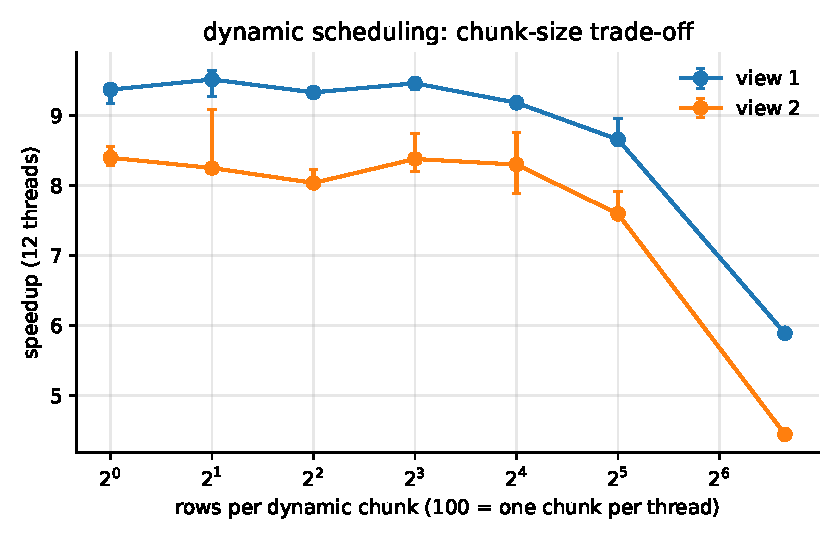
\includegraphics[width=0.62\linewidth]{cpp_prog1_chunk.pdf}
\caption{动态调度的粒度：12 线程加速比随每次领取的行数变化。}
\label{fig:chunk}
\end{figure}

\subsection{SMT：两个硬件线程能顶几个核}

官方作业问超线程对 Mandelbrot 有没有用。\cref{fig:smt} 比较了同样线程数放在不同数量物理核上的耗时：
6 个线程放在 3 个物理核（每核 2 个 SMT 线程）上，标量版耗时 62.5 ms，放在 6 个独立核上为 56.3 ms，
即 3 个核借助 SMT 完成了 6 个核约 90\% 的工作。原因是 Mandelbrot 的内层循环是一条依赖链：
\texttt{zr*zr}、\texttt{zi*zi}、相加、比较、再更新 \texttt{zr}、\texttt{zi}，每一步都要等上一步的 4 周期乘法延迟，
一个线程只能用掉执行端口的一小部分；第二个 SMT 线程的依赖链正好填进空闲的周期。
这也说明了一个常被忽略的事实：SMT 的收益取决于代码是受延迟限制还是受吞吐限制，不是固定的 ``20\%--30\%''。

紫色柱给出了反面验证。双向量交错版（第~\ref{sec:prog3}~节）在单线程内就交错了两条独立依赖链，已经填掉了一部分空闲周期，
因此它从 SMT 得到的收益最少：从 6 个核挤到 3 个核（每核 2 个 SMT 线程）时，view~1 的耗时标量版增加 11\%、AVX-512 版增加 3\%，
双向量交错版增加 17\%；view~2 上交错版增加 45\%。12 线程挤到 6 个核时同样如此（交错版慢 54\%，单向量 AVX-512 慢 23\%）。
\textbf{SMT 与 ILP~\cite{volkov} 争夺的是同一批空闲发射槽}，二者的收益不能简单相乘。

\begin{figure}[H]
\centering
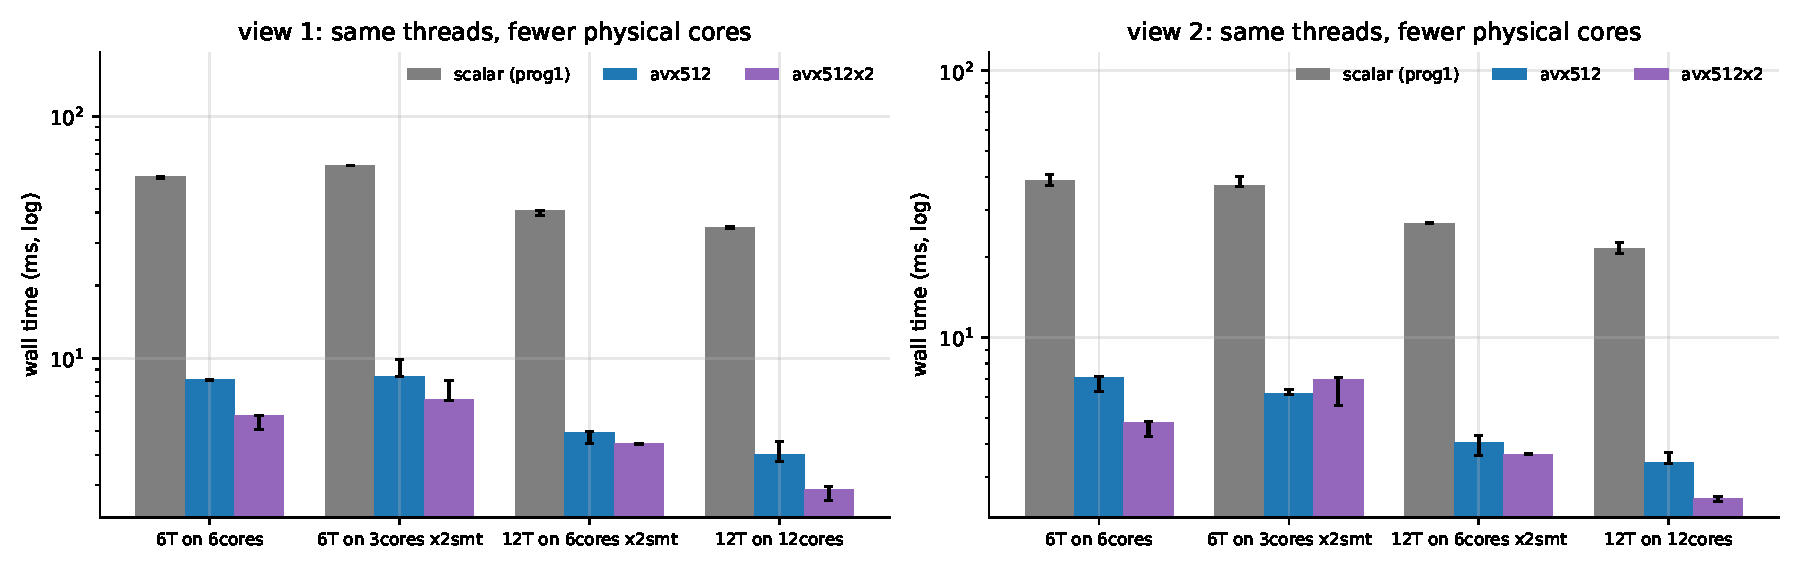
\includegraphics[width=\linewidth]{cpp_smt.pdf}
\caption{相同线程数、不同物理核数的耗时（对数坐标）。灰：标量 prog1 动态调度；蓝：AVX-512 task；紫：AVX-512 双向量交错 task。}
\label{fig:smt}
\end{figure}

\begin{findingbox}[：prog1]
Mandelbrot 的工作量集中在图像中部，连续块划分的加速比被最重的块限制（式~\ref{eq:blockbound}）；
隔行划分解决工作量不均，动态划分同时解决工作量不均和``慢核''问题。该内核受延迟限制，SMT 几乎能把一个核当两个用。
\end{findingbox}

%====================================================================
\section{Program 2：向量 intrinsics 与 lane 利用率}
\label{sec:prog2}

官方 prog2 提供一套``假''向量指令：每个操作带一个 mask，logger 记录发出的向量指令数和启用的 lane 数。
本文按同名 API 重写了 \texttt{cs149intrin.h}，\texttt{VECTOR\_WIDTH} 在编译期指定，分别编译 W=2/4/8/16 四个可执行文件。

\subsection{clampedExp}

\texttt{clampedExpVector} 的关键是用 mask 处理每个 lane 不同的指数：每次循环对仍有剩余指数的 lane 做一次乘法，
\texttt{\_cs149\_cntbits(maskActive)} 为 0 时退出；尾部 $N \bmod W$ 个元素用 \texttt{\_cs149\_init\_ones(rem)} 关掉。
lane 利用率为
\begin{equation}
U = \frac{\sum \text{每条指令启用的 lane 数}}{W \times \text{指令数}},
\end{equation}
一组 $W$ 个 lane 的循环次数由其中最大的指数决定，其余 lane 在后面几次循环里空转。

\begin{figure}[H]
\centering
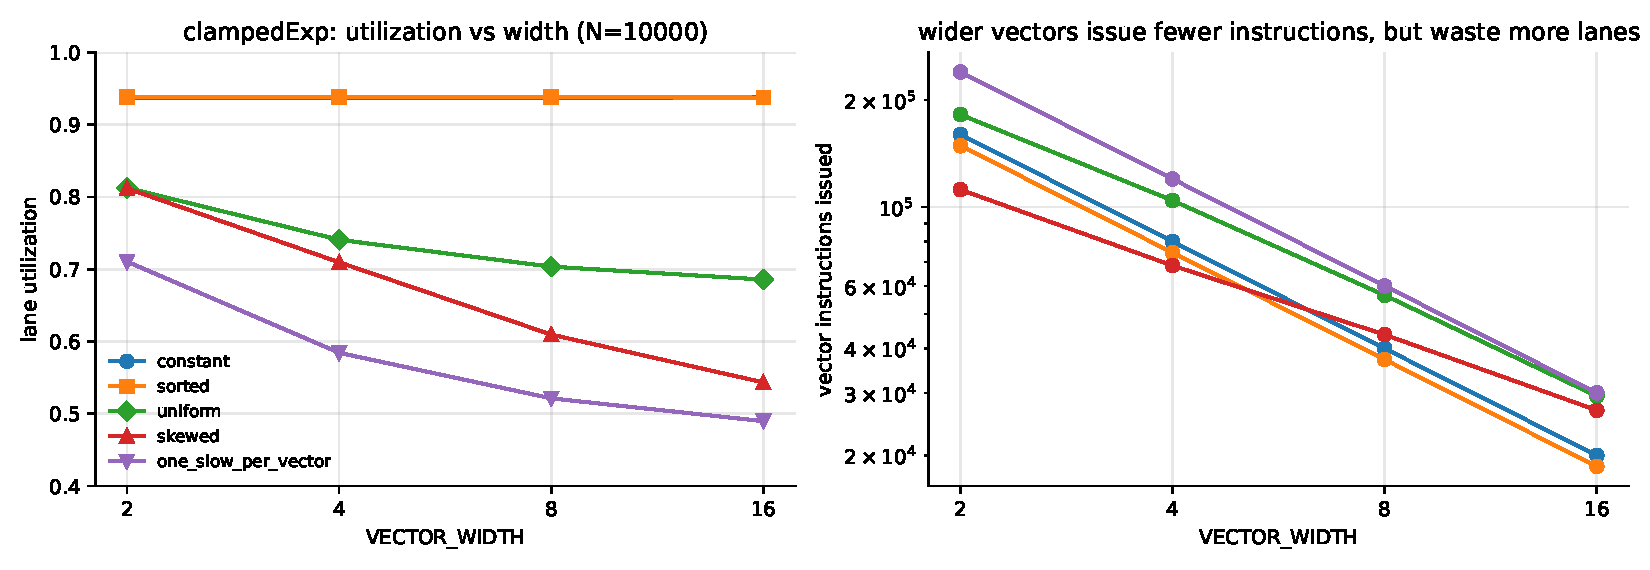
\includegraphics[width=\linewidth]{cpp_prog2_utilization.pdf}
\caption{左：lane 利用率随向量宽度的变化；右：发出的向量指令数。N=10000。}
\label{fig:prog2}
\end{figure}

\cref{fig:prog2} 和表~\ref{tab:prog2} 给出 5 种指数分布的结果：

\begin{table}[H]
\centering
\caption{clampedExp 的 lane 利用率（N=10000，指数取值 0--9）}
\label{tab:prog2}
\begin{tabular}{lcccc}
\toprule
指数分布 & W=2 & W=4 & W=8 & W=16 \\
\midrule
constant（全为 5） & 0.938 & 0.938 & 0.938 & 0.938 \\
sorted（均匀后排序） & 0.938 & 0.938 & 0.938 & 0.937 \\
uniform（官方设置） & 0.812 & 0.741 & 0.704 & 0.686 \\
skewed（10\% 为 9，其余为 1） & 0.812 & 0.710 & 0.610 & 0.543 \\
one\_slow\_per\_vector & 0.711 & 0.584 & 0.521 & 0.490 \\
\bottomrule
\end{tabular}
\end{table}

三点观察：

\begin{enumerate}
\item \textbf{均匀分布下利用率随宽度单调下降}：一组 lane 越多，组内最大指数越接近 9，空转越多。这正是官方问题的答案。
\item \textbf{constant 也不是 1}：每组 16 条指令里有一条是 \texttt{\_cs149\_vmove\_float(result, clampV, maskClamp)}，
$0.5$--$1.5$ 的 5 次方从不超过 9.999999，这条指令启用 0 个 lane，所以利用率恰为 $15/16 = 0.9375$。
\item \textbf{排序几乎消除了发散}：把同样的数据按指数排序后，相邻元素指数相同，利用率回到 0.938。
这对应 GPU 上的``按工作量对线程重排''（例如光线追踪中的 ray sorting、MoE 中按专家分组 token）。
\end{enumerate}

\subsection{arraySum}

\texttt{arraySumVector} 先用 $N/W$ 次向量加法得到 $W$ 个部分和，再做 $\log_2 W$ 轮 \texttt{hadd} + \texttt{interleave} 把它们归约到第 0 个 lane。
指令数为 $1 + 2N/W + 2\log_2 W$（一次清零、每个向量一次 load 与一次 add、每轮归约两条），实测与公式完全一致
（W=16、N=10000 时 1259 条），利用率为 1，相对误差 $<10^{-6}$（浮点加法顺序不同）。

%====================================================================
\section{Program 3：SIMD gang 与 task}
\label{sec:prog3}

\subsection{手写 gang：AVX2、AVX-512 与双向量交错}

ISPC 把一个函数编译成 $W$ 个 program instance 同时执行，发散的 lane 用 mask 关掉。本文用 intrinsics 直接写出这一过程：
每次处理同一行相邻的 8（AVX2）或 16（AVX-512）个像素，维护一个活跃 mask，所有 lane 都逃逸后跳出循环。
AVX-512 的比较直接产生 \texttt{\_\_mmask16}，计数用 \texttt{\_mm512\_mask\_add\_epi32}；AVX2 需要把比较结果当作 $-1$ 整数相减，
并用 \texttt{movemask} 判断是否全部结束。

\begin{lstlisting}[language=C++,caption={AVX-512 gang 的内层循环（\texttt{prog3\_mandelbrot\_simd/main.cpp}）}]
for (int k = 0; k < p.max_iter; ++k) {
    __m512 zr2 = _mm512_mul_ps(zr, zr), zi2 = _mm512_mul_ps(zi, zi);
    active = _mm512_mask_cmp_ps_mask(active, _mm512_add_ps(zr2, zi2), four, _CMP_NGT_UQ);
    if (!active) break;                          // every lane escaped
    cnt = _mm512_mask_add_epi32(cnt, active, cnt, one);
    __m512 ni = _mm512_mul_ps(_mm512_mul_ps(two, zr), zi);
    zr = _mm512_add_ps(cr, _mm512_sub_ps(zr2, zi2));
    zi = _mm512_add_ps(ci, ni);
}
\end{lstlisting}

每个 gang 的代价是组内最大迭代数，因此模型加速比为 $W\cdot U_W$，其中
\begin{equation}
U_W = \frac{\sum_i (c_i+1)}{\sum_{\text{gang}} W\,(\max_{i\in\text{gang}} c_i+1)}
\end{equation}
可由参考图像直接算出（view~1：$U_8 = 0.957$、$U_{16}=0.929$；view~2：$U_8=0.831$、$U_{16}=0.741$）。\cref{fig:simd} 比较实测与模型：

\begin{figure}[H]
\centering
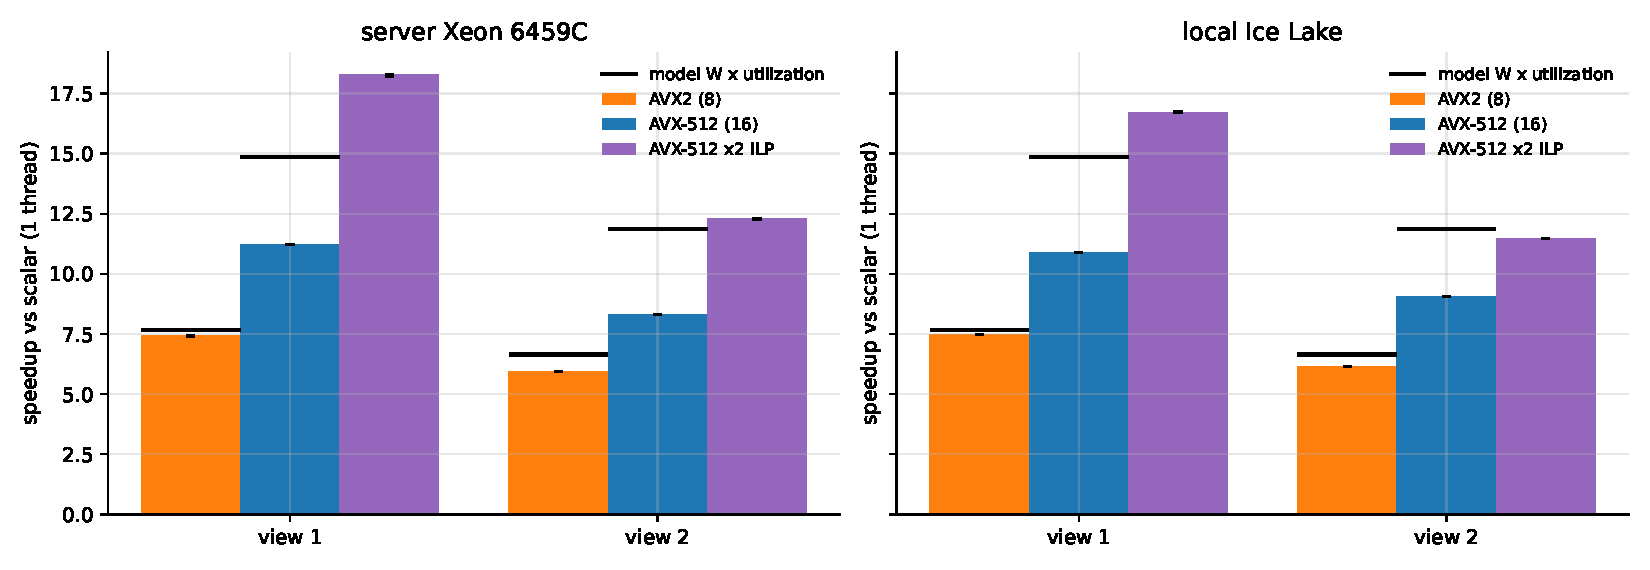
\includegraphics[width=\linewidth]{cpp_prog3_simd.pdf}
\caption{单线程 SIMD 加速比（相对标量）。黑线为模型 $W\cdot U_W$；紫色为 AVX-512 双向量交错。}
\label{fig:simd}
\end{figure}

\begin{itemize}
\item AVX2 实测 7.42 倍，模型 7.66 倍，二者接近：8 lane 版的瓶颈就是发散。view~2 为 5.96 倍，模型 6.65 倍。
\item AVX-512 实测 11.2 倍，比模型的 14.9 倍低得多。每次迭代除了 6 个浮点运算，还有比较、mask 计数、分支，
而依赖链长度与标量完全相同：16 个 lane 只是让每条依赖链``更宽''，没有让它``更短''。
\item 双向量交错（每次推进两组独立的 16 lane，\texttt{avx512x2}）达到 18.3 倍，超过 16 lane 的宽度。
两条独立依赖链交错发射，正好把 SMT 实验中观察到的空闲周期在单线程内填满。这是面试里``为什么 SIMD 加速可以超过 W''的标准例子：
标量基线本身没有吃满流水线，提高 ILP 的收益与 SIMD 宽度相乘。
\end{itemize}

\subsection{task 数量}

ISPC 的 \texttt{launch[n]} 把工作切成 $n$ 个 task 交给线程池。\cref{fig:tasks} 在 12 个工作线程上扫描 $n$：
$n < 12$ 时只有 $n$ 个核在干活；$n = 12$、16 时每个 task 是连续的一大块行，又回到了连续块划分的不均衡；
$n \ge 64$ 后加速比稳定在约 7.0（AVX-512）--7.6（双向量交错） 倍（相对同一 ISA 的单线程）。这说明 task 数应当远多于核数，
让线程池在运行时做负载均衡——官方答案通常给出``几十到几百个 task''，原因就在此。

\begin{figure}[H]
\centering
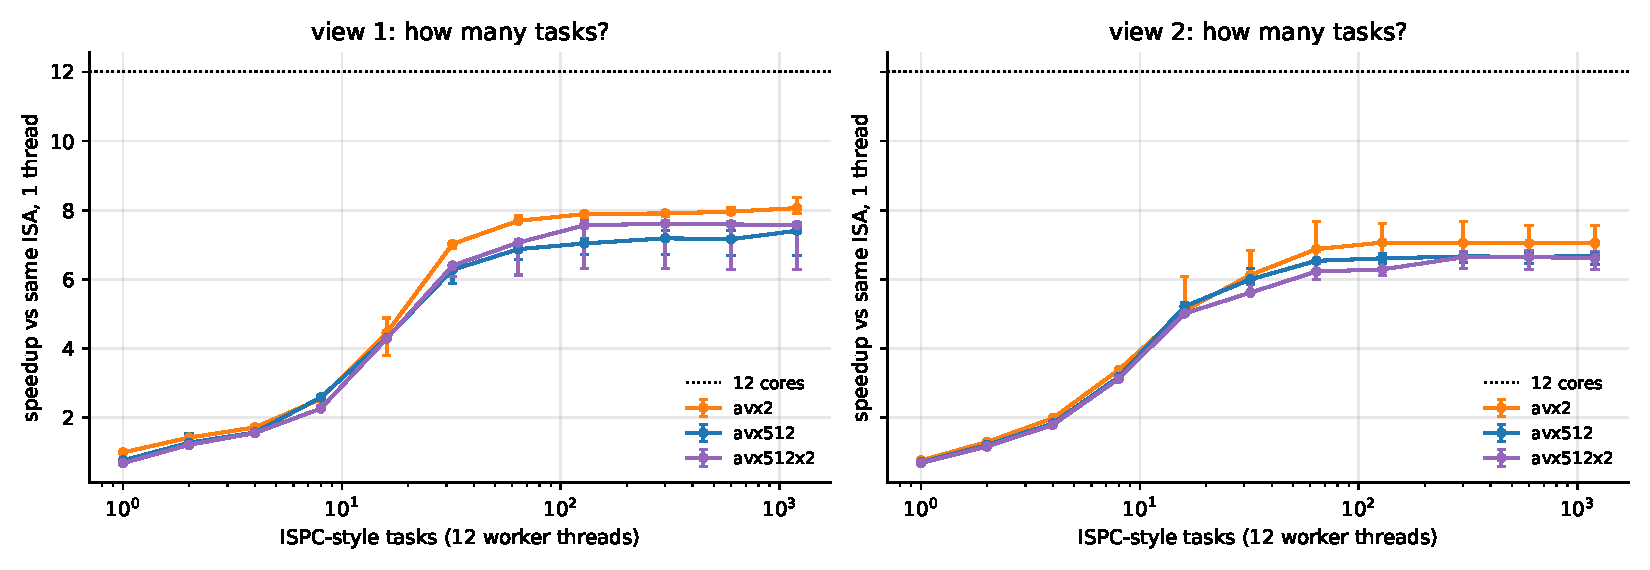
\includegraphics[width=\linewidth]{cpp_prog3_tasks.pdf}
\caption{ISPC 式 task 数量扫描（12 个工作线程）：相对同一 ISA 单线程的加速比。}
\label{fig:tasks}
\end{figure}

\subsection{把 SIMD、ILP、多核和 GPU 乘起来}

\cref{fig:ladder} 把 view~1/2 上每一步的加速画成``阶梯''：标量 $\to$ AVX2 $\to$ AVX-512 $\to$ 双向量交错 $\to$ 12 核 $\to$ RTX 5090。
CPU 上各级加速基本相乘：SIMD 约 11 倍、ILP 约 1.6 倍、12 核约 7.6 倍，合计约 139 倍（view~1）与 82 倍（view~2）。
RTX 5090 在同样 $1600\times1200$ 的图像上达到 8233 倍与 5762 倍，图像放大 16 倍、摊薄 launch 开销后为 10645 倍与 8267 倍，
即比最好的 12 核 CPU 版本再快 60--100 倍；第~\ref{sec:gpu}~节解释这个差距从哪里来。

\begin{figure}[H]
\centering
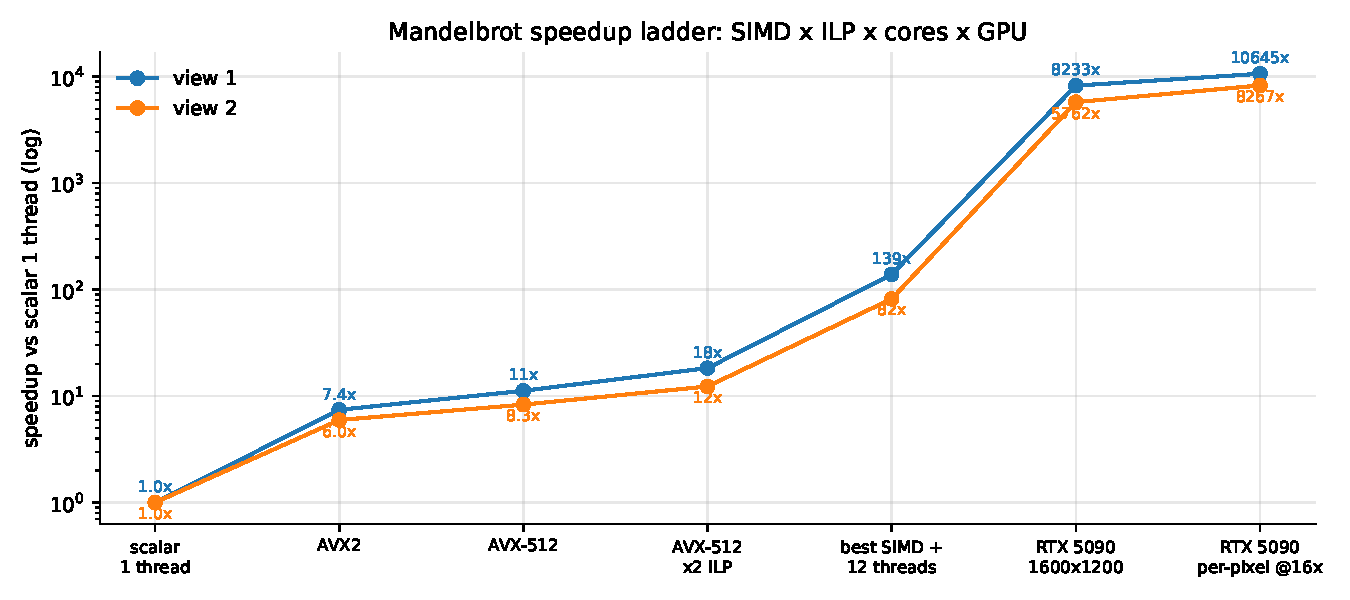
\includegraphics[width=\linewidth]{cpp_ladder.pdf}
\caption{Mandelbrot 加速阶梯（相对标量单线程，对数坐标）。}
\label{fig:ladder}
\end{figure}

\subsection{一个测量陷阱：worker 放在哪个 CPU 上}

扫描 task 时发现，``1 个 task、1 个工作线程''比在主线程上直接调用同一个函数指针慢约 23\%（相对速度 0.77）。最初怀疑是工作线程绑在了
承担中断的 CPU~0 上，于是对比了绑在 CPU~0、绑在另一个核、不绑核三种情况（\cref{fig:pin}）：三者在 3 轮中的 8 次里都是 0.77 左右，
只有 1 次接近 1.0，\textbf{假设被否定}。剩下的区别是工作线程每次计时都新建，而主线程刚刚连续跑过多次同样的内核；
这与上一节粒度扫描中观察到的``冷核''现象一致。
再看绝对值：view~1 的工作线程比主线程多 8.9\,ms（38.6 对 29.7\,ms），view~2 同样多 8.9\,ms（31.3 对 22.4\,ms）。
两种视角的工作量差 1.3 倍，多出来的时间却相同，所以这是每次 launch 一个\textbf{加性}的固定代价，而不是工作线程整体跑得慢。
本机 4 核上同样的实验给出不同的图景：绑在 CPU~0 时相对速度 0.75 / 0.90，绑在其他核或不绑核时 0.92--1.00，即本机只有 CPU~0 慢（推测与中断集中投递到 CPU~0 有关，未验证）。
A2 报告用 CPU 时间进一步区分了``等待''与``执行变慢''，结论是服务器上的 worker 在没有线程自旋时每条指令更贵，最可能的原因是宿主机的频率与空闲管理，
没有 \texttt{turbostat} 无法最终确认。
它的影响是\cref{fig:tasks} 中``相对单线程 SIMD''的加速比被系统性低估约 20\%，
而``相对标量''的数字（\cref{fig:ladder}）不受影响，因为标量基线也在主线程上测量、阶梯图只比较墙钟时间。
更稳妥的做法是像 prog5 那样使用常驻线程池，本文在 prog3 中保留了每次新建线程的实现，以便与官方 ISPC task 的语义对应。

\begin{figure}[H]
\centering
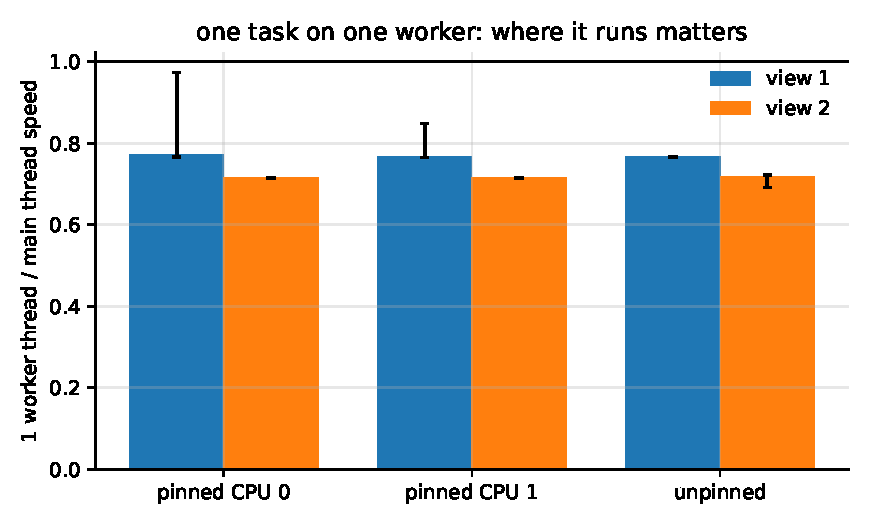
\includegraphics[width=0.62\linewidth]{cpp_pin.pdf}
\caption{1 个 task 在 1 个工作线程上运行时相对主线程的速度，按绑核位置区分。}
\label{fig:pin}
\end{figure}

%====================================================================
\section{Program 4：Newton sqrt 与最好、最坏输入}
\label{sec:prog4}

prog4 用 Newton 法求 $1/\sqrt{x}$，初值为 1，误差阈值 $10^{-5}$。迭代次数完全由输入决定（\cref{fig:prog4} 左）：
$x=1$ 时 0 次，$x\to 3$ 时约 20 次，$x\to 0$ 时更多。于是：

\begin{itemize}
\item \textbf{最好输入}（all\_slow，全部为 2.998）：每个元素都要 20 次迭代，没有发散，计算量大到足以摊薄 load/store；
AVX-512 达到 13.5 倍，再乘 12 线程达到 104 倍。
\item \textbf{最坏输入}（one\_slow\_W，每 W 个元素中 1 个为 2.998、其余为 1.0）：每个向量都必须跑满 20 次，有效工作只有 $1/W$。
AVX2 在 one\_slow\_8 上只有 0.72 倍——\textbf{比标量还慢}，这正是官方要求构造的情形。
\end{itemize}

\begin{figure}[H]
\centering
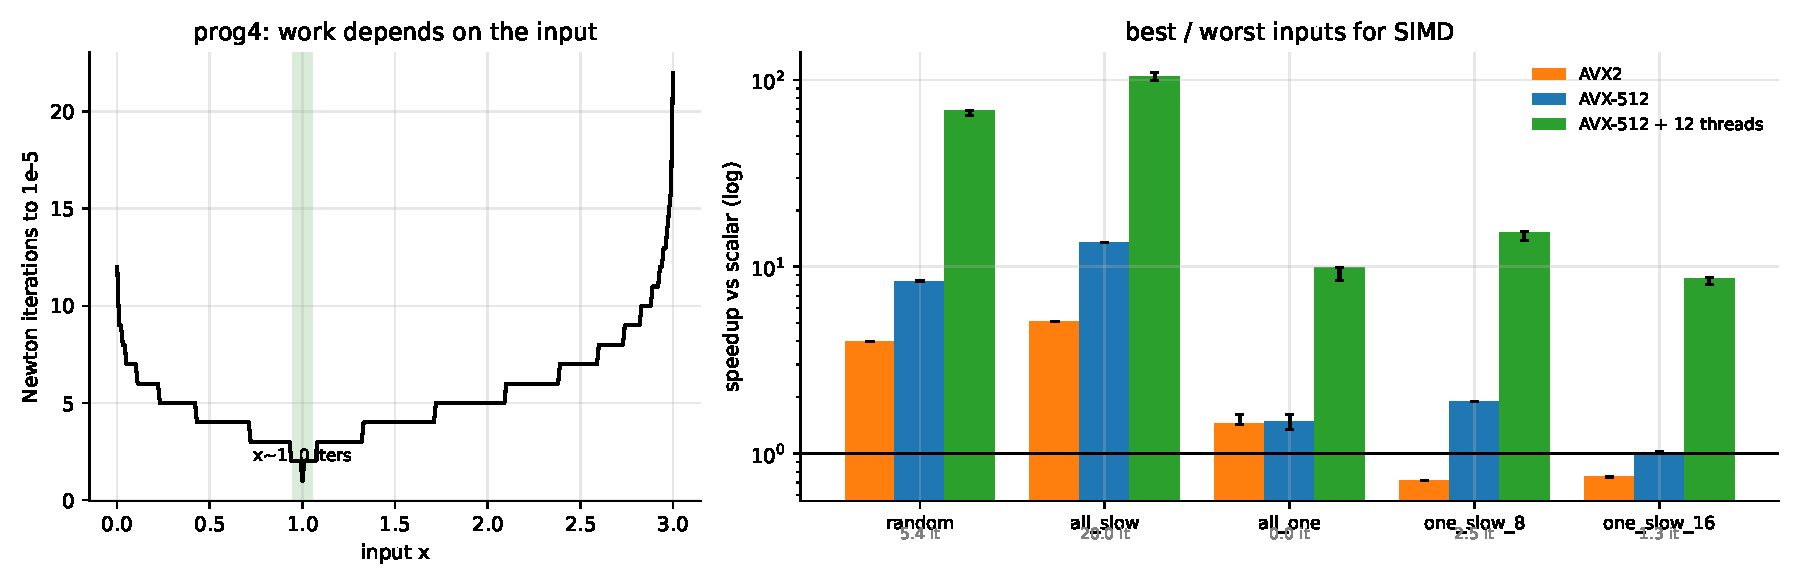
\includegraphics[width=\linewidth]{cpp_prog4_sqrt.pdf}
\caption{左：迭代次数随输入的变化；右：各输入模式的加速比（对数坐标），灰字为平均迭代次数。}
\label{fig:prog4}
\end{figure}

表~\ref{tab:prog4} 列出耗时。最能说明发散代价的是 AVX-512 一列：all\_slow、one\_slow\_8、one\_slow\_16 三种输入的平均迭代次数是
20、2.5、1.25，耗时却分别为 96.8、96.8、97.3~ms，几乎完全相同；AVX2 在 all\_slow 与 one\_slow\_8 上也同为 256~ms。
对 SIMD 而言，一个向量的代价只取决于其中最慢的 lane。

\begin{table}[H]
\centering
\caption{prog4 耗时（N = 2000 万，服务器 3 轮中位数）}
\label{tab:prog4}
\begin{tabular}{lrrrrrr}
\toprule
输入 & 平均迭代 & 标量 ms & AVX2 ms & AVX-512 ms & AVX-512 加速 & +12 线程 \\
\midrule
random & 5.35 & 742.7 & 186.8 & 88.9 & 8.36 & 68.5 \\
all\_slow & 20.0 & 1305.5 & 256.2 & 96.8 & 13.48 & 104.1 \\
all\_one & 0.0 & 13.3 & 9.1 & 9.0 & 1.48 & 9.9 \\
one\_slow\_8 & 2.50 & 183.3 & 256.1 & 96.8 & 1.89 & 15.2 \\
one\_slow\_16 & 1.25 & 99.0 & 131.7 & 97.3 & 1.02 & 8.6 \\
\bottomrule
\end{tabular}
\end{table}

两个值得追问的细节：

\begin{enumerate}
\item \textbf{为什么 AVX-512 比 AVX2 快 2.6 倍而不是 2 倍？}AVX2 没有 mask 寄存器，冻结已收敛的 lane 要用 \texttt{blendv}（2 个 uop），
判断是否全部收敛要 \texttt{movemask}；AVX-512 的比较直接写 mask，更新用 \texttt{mask\_mov}。每次迭代的指令更少。
\item \textbf{为什么 AVX2 在 all\_slow 上只有 5.1 倍？}标量 all\_slow 每个元素每次迭代平均 $1305.5\,\text{ms}/(2\times10^7\times20)=3.3$~ns，
约 11 个周期，而一次迭代的依赖链（3 次乘、1 次减、1 次乘）约 20 个周期。差距说明乱序执行在预测正确的 20 次循环后
提前开始了下一个元素，让两个元素的依赖链重叠——标量基线自带约 2 倍的 ILP，这部分在 SIMD 版本里没有，因而加速比打了折扣。
\end{enumerate}

%====================================================================
\section{Program 5：saxpy 与内存带宽}
\label{sec:prog5}

saxpy 计算 $r = a x + y$，每个元素 2 次浮点运算、读 8 字节、写 4 字节，算术强度 $I = 2/12 \approx 0.17$~FLOP/B。
在 roofline~\cite{roofline} 模型
\begin{equation}
P = \min(P_{\text{peak}},\; I \cdot B)
\end{equation}
里，$I$ 远小于任何 CPU 的拐点（约 10--50~FLOP/B），因此性能完全由带宽 $B$ 决定。

\subsection{带宽随工作集的变化}

\cref{fig:bwsize} 扫描工作集（三个数组总大小）。单线程时，工作集小于 L1（48~KB）的 SIMD 内核达到约 229~GB/s，
进入 L2 后约 125~GB/s，超过 L2（2~MB）后跌到 35~GB/s，超过 L3 后只剩约 18~GB/s。12 线程时 L2 容量相当于 $12\times2$~MB，
工作集 12.6~MB 时总带宽超过 1~TB/s；超过 L3 后降到 130~GB/s 左右。曲线的左端 12 线程反而很低：每次调用只有几微秒，
线程池同步的开销占了主导——\textbf{小问题不值得并行}。

\begin{figure}[H]
\centering
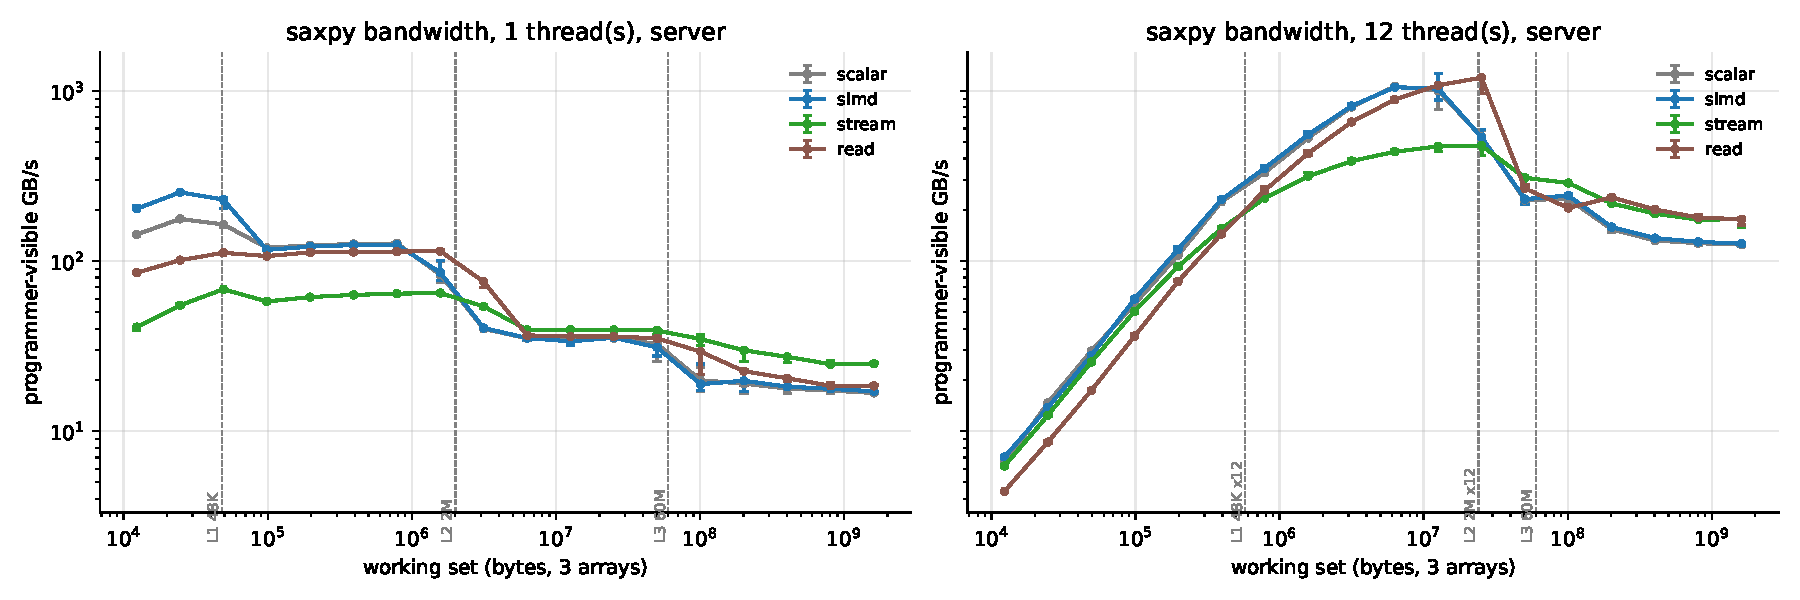
\includegraphics[width=\linewidth]{cpp_prog5_sizes.pdf}
\caption{saxpy 程序员可见带宽（12~B/元素）随工作集变化，虚线为各级缓存容量（多线程时按线程数放大私有缓存）。}
\label{fig:bwsize}
\end{figure}

\subsection{write-allocate 与 streaming store}

普通 store 写入一个不在缓存中的行时，CPU 先把整行读进来（read-for-ownership），因此 saxpy 的真实 DRAM 流量是 16~B/元素，
而不是程序员看到的 12~B。\texttt{\_mm512\_stream\_ps} 是 non-temporal store，绕过缓存直接写内存，省掉这次读，流量回到 12~B/元素。
DRAM 区间的结果符合这个账：单线程 stream 的可见带宽 25~GB/s，普通 SIMD 18~GB/s，比值 1.39；12 线程 175 对 130~GB/s，比值 1.35，
都接近 $16/12 = 1.33$。但在缓存区间 stream 很差（单线程 L1 区间 68 对 229~GB/s）：数据本可以留在缓存里，non-temporal store
却强行写回内存。结论是 streaming store 只适合``写完很久不再读''的大数组。

\subsection{线程扩展与 NUMA}

\cref{fig:bwthreads} 左图是 768~MB 工作集的真实 DRAM 带宽~\cite{stream}（含 write-allocate~\cite{drepper}）随线程数的变化：单线程 23~GB/s，12 线程 173~GB/s，
几乎线性增长，尚未饱和。这与官方作业在四核桌面机上看到的``两三个线程就饱和''不同：Sapphire Rapids 每路 8 个 DDR5 通道，
单核受限于自己能挂起的 cache miss 数（Little~\cite{hp} 定律：带宽 = 并发请求数 $\times$ 64~B / 延迟），而不是内存控制器。
本机四核虚拟机同样未饱和（4 线程约 59~GB/s）。

\begin{figure}[H]
\centering
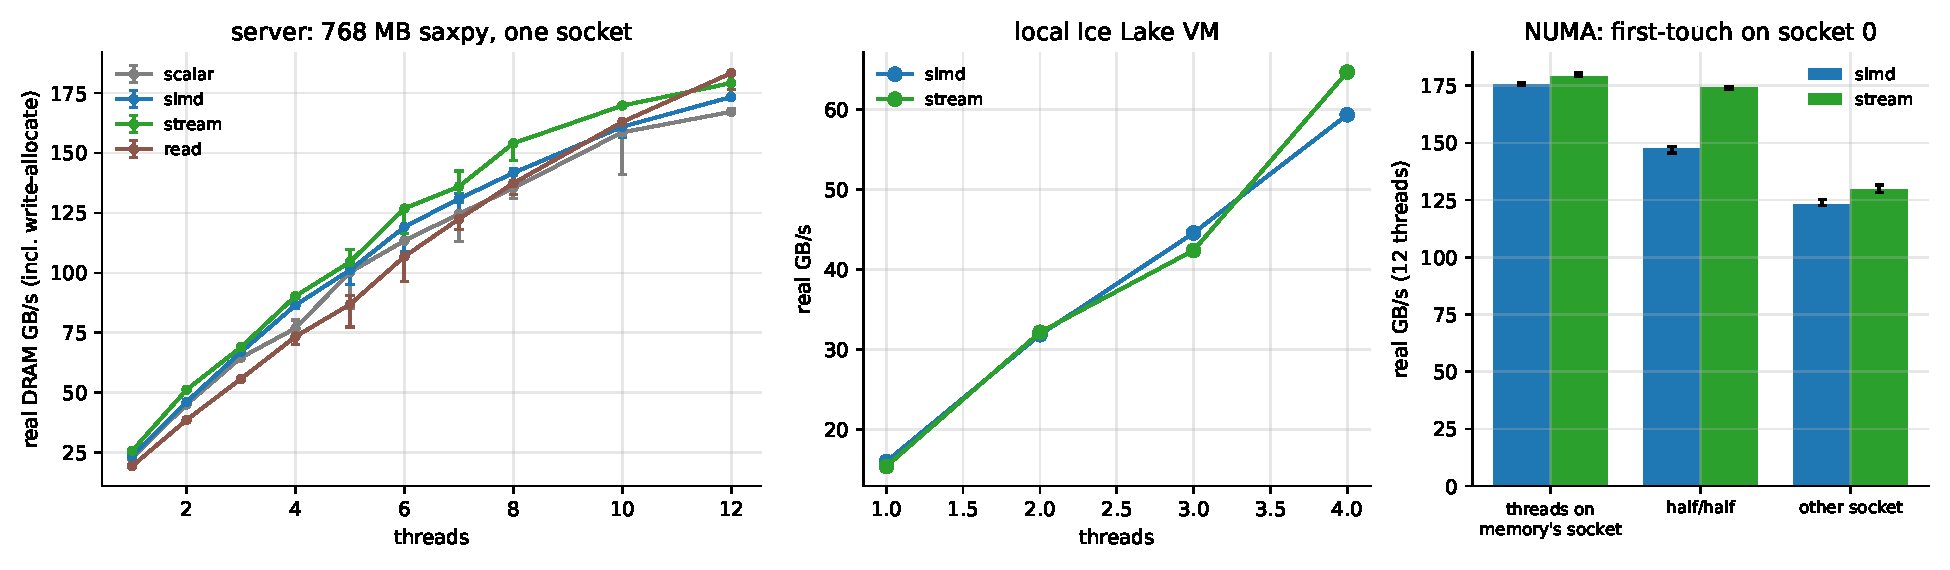
\includegraphics[width=\linewidth]{cpp_prog5_threads.pdf}
\caption{左：服务器 DRAM 带宽随线程数变化；中：本机；右：NUMA 放置（数据由主线程 first-touch 在 socket~0）。}
\label{fig:bwthreads}
\end{figure}

右图是 NUMA 实验：数组由主线程初始化，按 first-touch 策略全部落在 socket~0 的内存上。12 个线程都在 socket~0 时
SIMD 内核 175~GB/s，全部在 socket~1 时 123~GB/s（下降 30\%），各一半时 147~GB/s。在双路服务器上做内存密集计算，
数据初始化也要并行化，并让每个线程初始化自己将要处理的那一段。

%====================================================================
\section{Program 6：K-means 的 profiling 与优化}
\label{sec:prog6}

官方 prog6 给出一个慢的 K-means（M = 100 万个点、N = 100 维、K = 3），要求先计时找瓶颈再优化。baseline 照搬官方结构：
\texttt{computeAssignments} 外层循环 K、内层循环 M，计算带 \texttt{sqrt} 的欧氏距离；\texttt{computeCentroids} 和 \texttt{computeCost} 串行。
数据由 8 个高斯簇生成，收敛需要 3 轮迭代。\cref{fig:kmeans} 是分阶段耗时：

\begin{figure}[H]
\centering
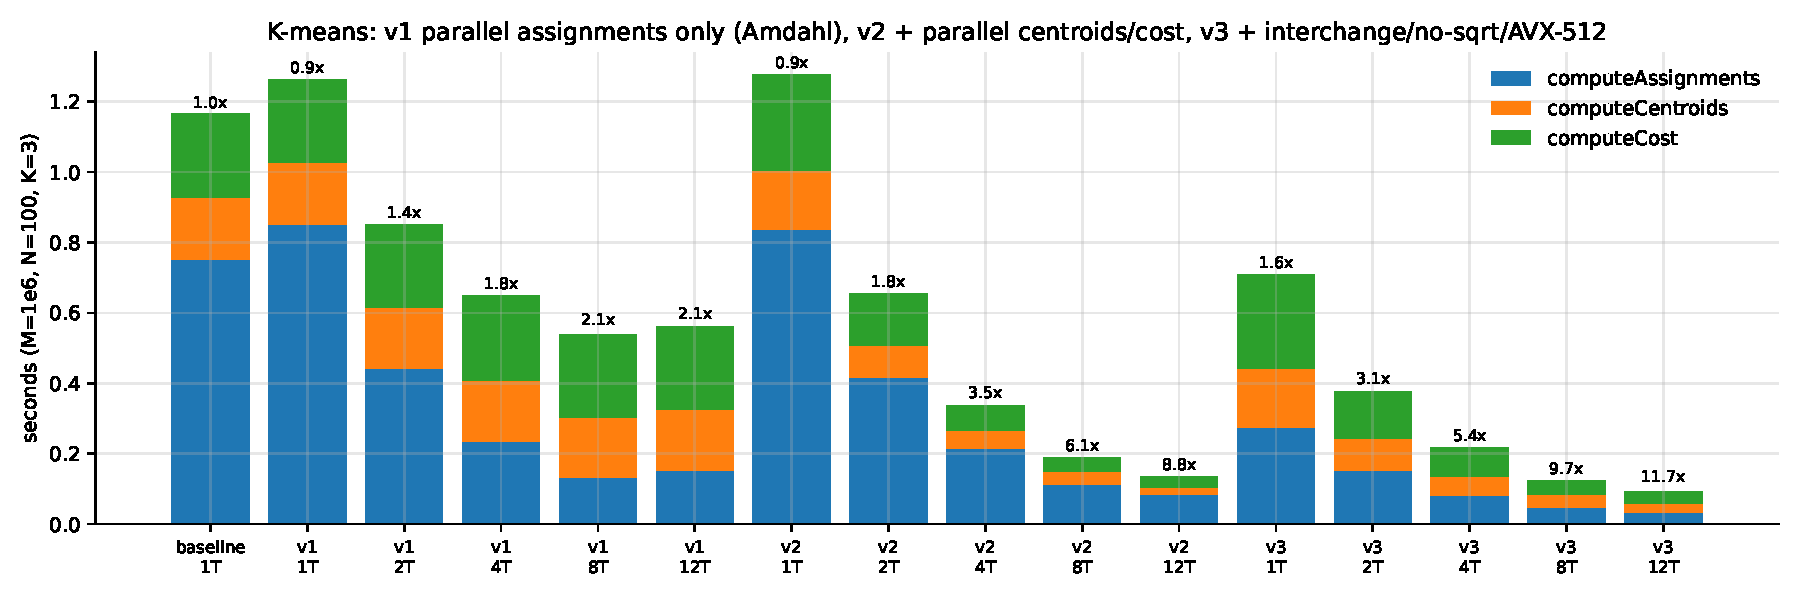
\includegraphics[width=\linewidth]{cpp_prog6_kmeans.pdf}
\caption{K-means 分阶段耗时与加速比（服务器 3 轮中位数）。}
\label{fig:kmeans}
\end{figure}

\begin{itemize}
\item \textbf{baseline}：总计 1.163~s，其中 \texttt{computeAssignments} 0.752~s（65\%），\texttt{computeCentroids} 0.176~s，\texttt{computeCost} 0.238~s。
\item \textbf{v1（官方期望的改法）}：按点 $m$ 把 \texttt{computeAssignments} 分给 $T$ 个线程。8 线程时该阶段降到 0.131~s，
但另两个阶段仍是 0.41~s，总加速只有 2.1 倍。Amdahl~\cite{amdahl} 定律给出的上限是 $1/(1-0.65) = 2.8$ 倍。
\item \textbf{v2}：\texttt{computeCentroids} 和 \texttt{computeCost} 也按点并行，每个线程累加到私有的部分和，最后合并（避免对共享数组的原子操作和 false sharing）。12 线程 8.8 倍。
\item \textbf{v3}：三处单线程优化——(a) 循环交换为外层 $m$、内层 $k$，每个点只从内存读一次（baseline 每个点读 K 次，共 2.4~GB）；
(b) 比较平方距离，省掉 \texttt{sqrt}（单调函数不改变 argmin）；(c) AVX-512 计算距离。单线程即达 1.64 倍，12 线程 11.7 倍。
\end{itemize}

所有版本的聚类分配与 baseline 完全一致（mismatch = 0），迭代次数相同。v3 在 8 线程以后 \texttt{computeAssignments} 每轮约 15~ms，
相当于每秒读约 55~GB 数据，已接近这一阶段的带宽与线程启动开销的组合上限。

%====================================================================
\section{GPU 对照：同样的三个问题在 SIMT 上}
\label{sec:gpu}

GPU 的 warp 就是一个 32 lane 的 gang，只是由硬件维护 mask。把 prog3/4/5/6 的内核写成 CUDA（\texttt{gpu/a1\_gpu.cu}），
可以检验 CPU 上得到的结论哪些成立、哪些不成立。

\subsection{Mandelbrot：warp 效率与 occupancy}

一个线程计算一个像素，warp 由 block 内连续的 32 个线程组成。block 形状决定一个 warp 覆盖的是一行 32 个像素还是一个 $8\times4$ 的小方块，
后者的像素空间相关性更强，warp 执行效率更高。\cref{fig:gpumandel} 在 $6400\times4800$ 的图像上扫描 12 种形状：

\begin{figure}[H]
\centering
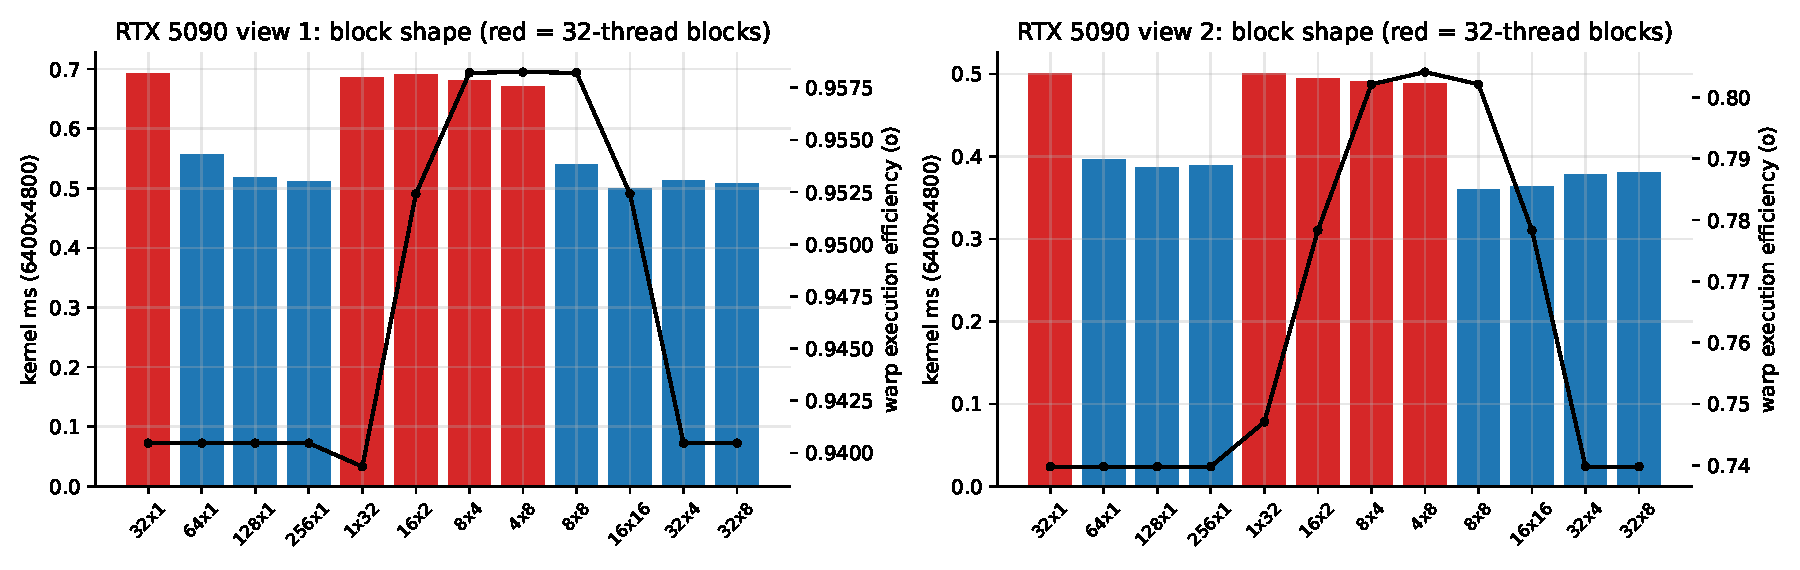
\includegraphics[width=\linewidth]{cpp_gpu_mandel_shapes.pdf}
\caption{RTX 5090 上 block 形状对 kernel 时间（柱）与 warp 执行效率（点线）的影响；红色柱为每个 block 只有 32 个线程的形状。}
\label{fig:gpumandel}
\end{figure}

\begin{itemize}
\item 2D 方块的 warp 效率更高（view~1：$8\times4$ 为 0.958，$32\times1$ 为 0.940；view~2：0.802 对 0.740），与 prog2 中``排序减少发散''是同一个道理。
\item 但每个 block 只有 32 个线程的形状（红色）都慢：每个 SM 能驻留的 block 数有上限（sm\_120 为 32 个），32 线程的 block 让每个 SM 最多只有 1024 个线程，
可用于隐藏延迟的 warp 不够。$8\times8$ 与 $16\times16$ 兼顾了空间局部性和 occupancy，是最快的两种（view~2 为 0.360~ms 与 0.364~ms，$32\times1$ 为 0.501~ms）。
\end{itemize}

\subsection{sqrt：GPU 上发散为什么``不见了''}

同一个 Newton sqrt 在 RTX 5090 上处理 2000 万个元素，所有输入模式的耗时都在 0.096--0.108~ms 之间（\cref{fig:gpusqrt} 右）。
读写 160~MB 用 0.104~ms，相当于 1.54~TB/s——kernel 被显存带宽限制，计算（即使是发散的计算）被完全隐藏。
把每个元素的求解重复 $R$ 次（初值略作扰动，避免被编译器消除），kernel 逐渐变成计算受限，发散的代价重新出现（\cref{fig:gpusqrt} 左）。$R=64$ 时：

\begin{itemize}
\item one\_slow\_8、one\_slow\_16、one\_slow\_32 的耗时（5.05、5.04、5.03~ms）与 all\_slow（5.03~ms）完全相同：warp 宽 32，只要每 32 个元素里有一个慢元素，整个 warp 都要跑满 20 次迭代。
这与 CPU 上 AVX-512 的 one\_slow\_16 结论一致，只是 GPU 的``gang''更宽。
\item one\_slow\_64 为 2.81~ms，约为 all\_slow 的一半：只有一半的 warp 含有慢元素。
\item random 为 3.35~ms，是 all\_slow 的 67\%，而平均迭代数只有 all\_slow 的 27\%（5.35 对 20）；把同样的数据排序后（sorted\_random）降到 1.59~ms，快 2.1 倍。
这就是 GPU 上``按工作量重排线程''的收益，对应 prog2 中排序把 lane 利用率从 0.69 提到 0.94。
\end{itemize}

这说明``发散有多贵''不是常数，取决于内核在 roofline 上的位置：同一个发散的内核，带宽受限时代价为零，计算受限时代价与 CPU 的 SIMD 完全相同。

\begin{figure}[H]
\centering
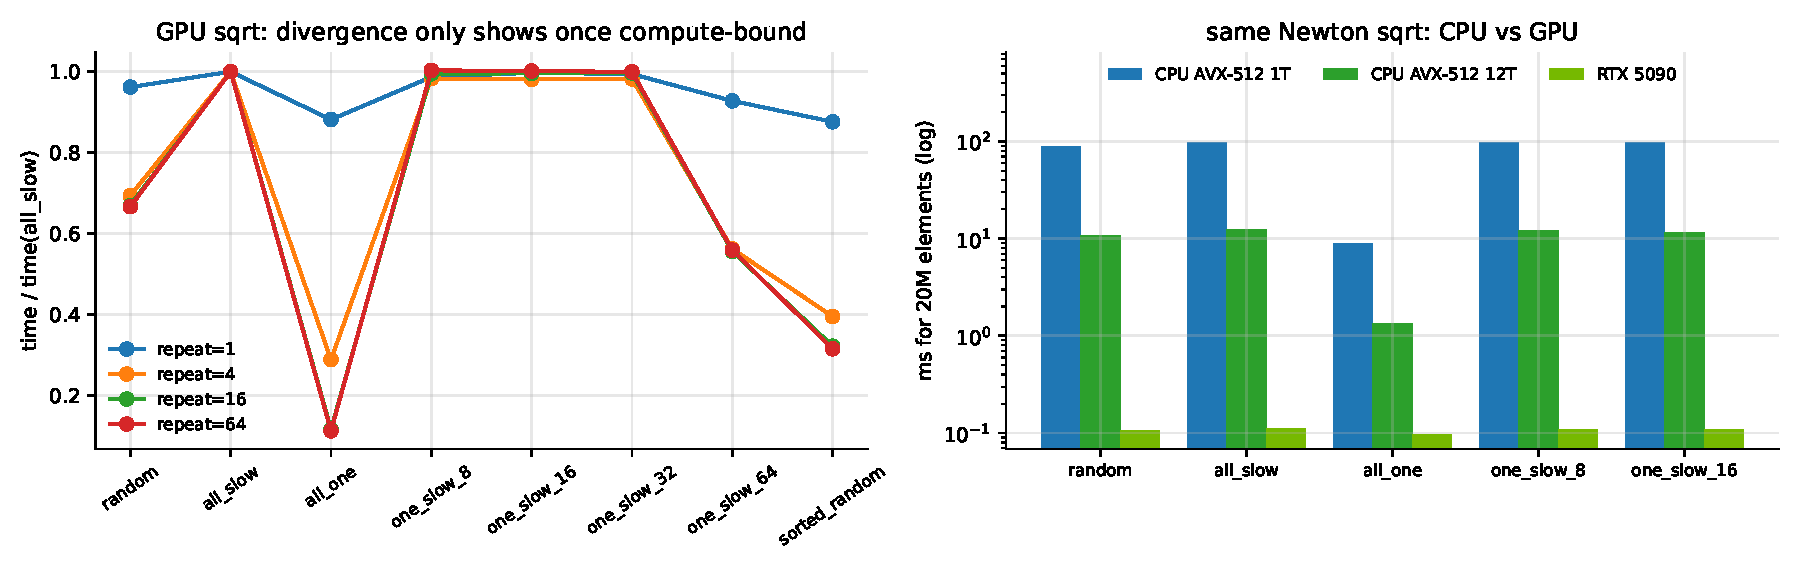
\includegraphics[width=\linewidth]{cpp_gpu_sqrt.pdf}
\caption{左：各输入相对 all\_slow 的耗时，$R$ 为每个元素重复求解的次数；右：同一 sqrt 在 CPU 与 GPU 上的耗时（2000 万元素）。}
\label{fig:gpusqrt}
\end{figure}

\subsection{saxpy：GPU 赢在显存，输在 PCIe}

\cref{fig:bwcmp} 把 GPU saxpy 与 CPU 放在同一坐标系：显存区间 GPU 稳定在约 1.55~TB/s（标称 1.79~TB/s 的 87\%），
L2（96~MB）区间峰值约 6.1~TB/s；一旦把输入从 host 拷到 device、再把结果拷回来，端到端只剩约 52~GB/s，
低于服务器 CPU 12 线程的 130~GB/s。这正是 CS149 Assignment 3 Part 1 要学生得出的结论：
\textbf{带宽受限的小算子不值得为它把数据搬上 GPU}，GPU 的优势要靠让数据常驻显存、把多个算子融合在一次搬运里。

\begin{figure}[H]
\centering
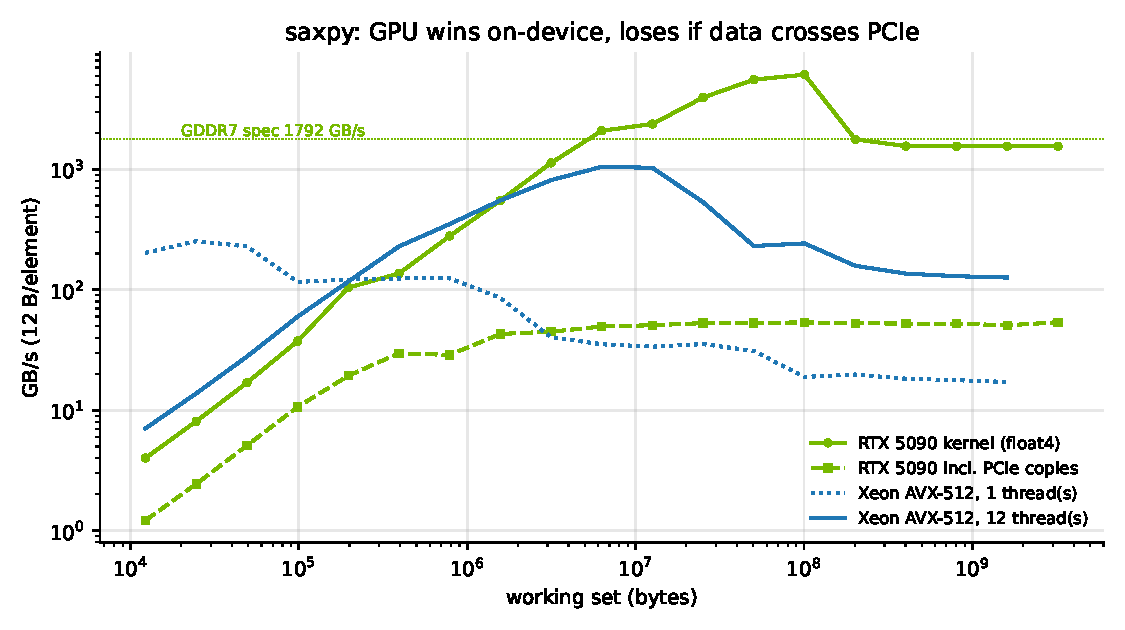
\includegraphics[width=0.8\linewidth]{cpp_bw_cpu_vs_gpu.pdf}
\caption{saxpy 带宽：RTX 5090（kernel、含 PCIe 拷贝）与 Xeon AVX-512（1 线程、12 线程）。}
\label{fig:bwcmp}
\end{figure}

\subsection{K-means 的 assignment kernel：合并访存}

在 GPU 上每个线程负责一个点。数据按点存储（AoS，$M\times N$）时，同一 warp 的 32 个线程在同一时刻读取相距 800~B 的地址，
无法合并；转置成按维存储（SoA，$N\times M$）后相邻线程读相邻地址。实测 AoS 3.74~ms（214~GB/s 有效带宽），SoA 1.43~ms（560~GB/s），
快 2.6 倍；结果与 CPU 参考逐个一致。相比 CPU v3 的 12 线程（每轮约 11~ms），GPU SoA 版本快约 8 倍。

\subsection{为什么 GPU 比 12 核 AVX-512 快 60--100 倍}

用``每秒能做多少 lane 运算''粗算：RTX 5090 有 170 个 SM，每个 SM 128 个 FP32 lane，频率约 2.4~GHz，约 $5.2\times10^{13}$ lane-op/s；
12 个 Xeon 核每核 2 个 512 bit 浮点端口、16 lane、约 3~GHz，约 $1.2\times10^{12}$ lane-op/s，峰值相差约 45 倍。
实测 GPU 每秒完成约 $4.5\times10^{12}$ 次有效的像素迭代（\cref{fig:gpuiters}），每次迭代约 8 个运算，即约 $3.6\times10^{13}$ op/s，达到峰值的约 70\%；
CPU 最好的版本比 GPU 慢 59 倍，折算约为自身峰值的 50\%。差距的第二个来源是延迟隐藏：GPU 每个 SM 同时驻留几十个 warp，一个 warp 等待乘法结果时调度器发射另一个 warp，
依赖链延迟几乎被完全隐藏；CPU 每个核只有 2 个硬件线程，依赖链延迟只能靠 SMT 和手工交错（第~\ref{sec:prog3}~节，约 1.6 倍）部分弥补。
\cref{fig:gpuiters} 还显示，迭代上限只有 64 时 GPU 吞吐明显偏低：kernel 只运行约 0.17~ms，launch 与尾部 wave 的开销占比大。

\begin{figure}[H]
\centering
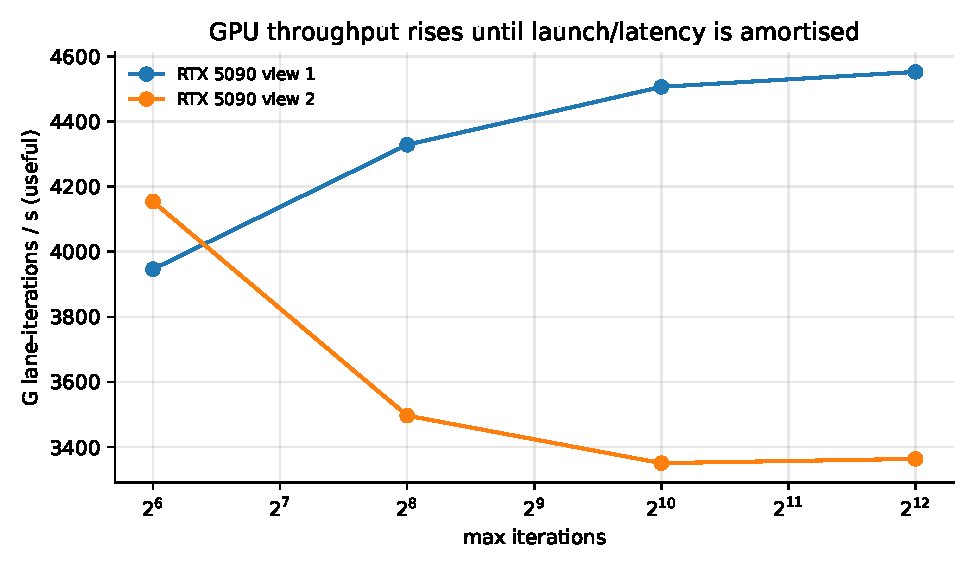
\includegraphics[width=0.62\linewidth]{cpp_gpu_iters.pdf}
\caption{RTX 5090 Mandelbrot（$6400\times4800$）有效迭代吞吐随最大迭代数的变化（取 12 种 block 形状中的最好值）。}
\label{fig:gpuiters}
\end{figure}

%====================================================================
\section{仓库原有 Python 版本的回顾}
\label{sec:python}

仓库最初用 Python/numpy 实现了 prog1/2/4/5 的核心问题（进程池代替线程、gang 利用率模型、numpy 掩码执行）。
\cref{fig:python} 是其中两张图。它们的定性结论与 C++ 版一致（连续块不均衡、发散代价、带宽很快饱和），但数字不能用于回答作业：
numpy 每次调用有固定开销，Python 版 Mandelbrot 的单像素代价与块大小有关（详见实验 README 中的``测量陷阱''），
而进程间通信又引入了与并行无关的开销。C++ 版的单线程 Mandelbrot（0.33~s）比 numpy 版（1.28~s）快约 4 倍，
SIMD 版快约 45 倍，这才是作业想要测量的东西。

\begin{figure}[H]
\centering
\begin{subfigure}{0.49\linewidth}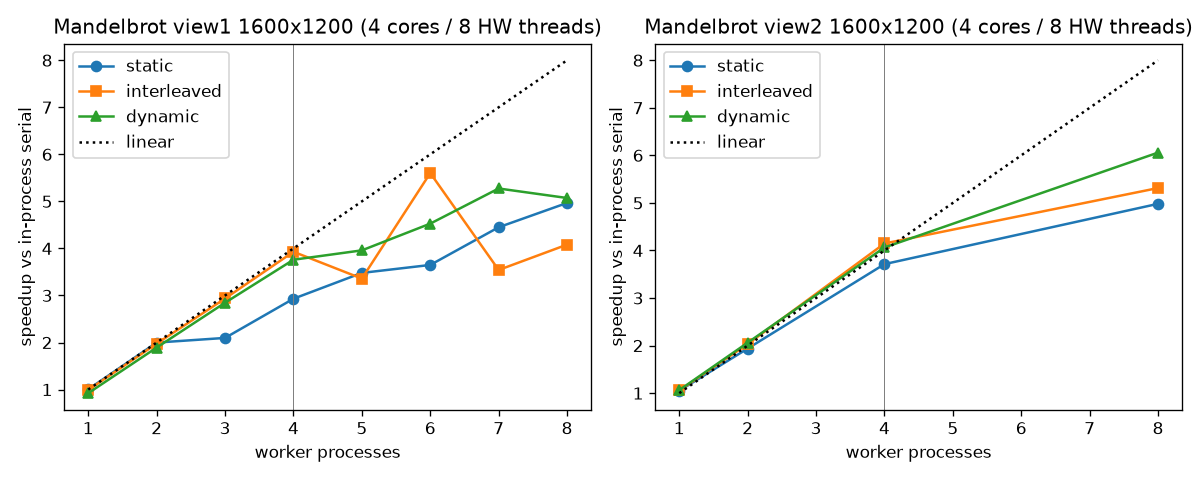
\includegraphics[width=\linewidth]{mandel_speedup.png}\caption{Python 进程池版 prog1}\end{subfigure}
\begin{subfigure}{0.49\linewidth}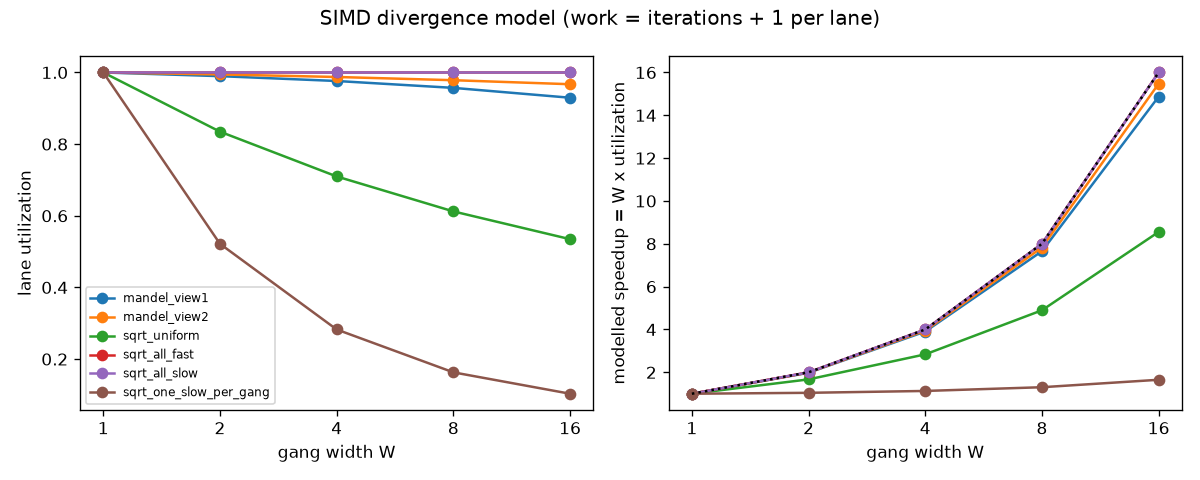
\includegraphics[width=\linewidth]{simd_utilization.png}\caption{gang 利用率模型}\end{subfigure}
\caption{仓库原有 Python 版本的结果（定性参考）。}
\label{fig:python}
\end{figure}

%====================================================================
\section{面试专题}
\label{sec:interview}

\subsection{20 秒版本}

并行加速有三个杀手：负载不均、SIMD 发散和带宽。Mandelbrot 中间贵，连续块划分 12 核只有 5.89 倍，动态分块 11.1 倍；
一个向量的代价由最慢的 lane 决定，sqrt 每 8 个元素混一个慢的，AVX2 就比标量还慢；saxpy 每 12 字节只做 2 次浮点运算，
单核只能拿到 23~GB/s，加核到 12 个也只有 173~GB/s，搬到 GPU 上如果要过 PCIe 只剩 52~GB/s。
另外，这个 Mandelbrot 内核受延迟限制，SMT 和 ILP 都能接近翻倍。

\subsection{追问与答案}

\begin{iqbox}{为什么 3 个线程比 2 个线程还慢？}
\textbf{答}：连续块划分时墙钟时间由最重的块决定。view~1 三等分时，中间那块包含整个 Mandelbrot 集主体，最重块的工作量是平均的 1.8 倍以上，
所以加速比只有约 1.6 倍，比 2 线程时两块对称（各约一半）还差。解决办法是隔行或动态划分。\\
\textbf{常见错答}：``线程创建开销''或``缓存冲突''。线程只创建 3 个，开销是微秒级；每线程计时图直接显示是工作量不均。
\end{iqbox}

\begin{iqbox}{超线程对 Mandelbrot 有用吗？}
\textbf{答}：有，而且接近翻倍。实测 6 个线程在 3 个物理核上的耗时只比 6 个独立核多约 11\%。原因是内层循环是一条乘加依赖链，
单线程每个周期只能发射很少的指令，另一个硬件线程的独立依赖链正好填满空闲端口。如果代码已经吃满执行端口（例如高度优化的 GEMM），SMT 的收益会接近 0。本文的双向量交错版就是证据：它在单线程内已经交错了两条依赖链，从 SMT 得到的收益明显少于单向量版。\\
\textbf{常见错答}：``超线程只有 20\%--30\% 收益''——这是平均值，不是规律；或者``超线程共享执行单元所以没用''。
\end{iqbox}

\begin{iqbox}{8 宽 SIMD 为什么 Mandelbrot 只有约 7.4 倍、而 16 宽只有约 11 倍？}
\textbf{答}：模型加速比是 $W\times U_W$，view~1 的 $U_8=0.957$、$U_{16}=0.929$，所以理论值是 7.66 和 14.9。AVX2 接近模型；AVX-512 还受依赖链延迟限制，
每次迭代的比较、mask 计数和分支也要占发射槽。在单线程里交错两组向量后 AVX-512 达到约 18.3 倍，超过 16。\\
\textbf{常见错答}：``AVX-512 降频''——Sapphire Rapids 上降频很小，双向量交错版同样用 512 bit 却快 1.6 倍，说明主因是延迟而不是频率。
\end{iqbox}

\begin{iqbox}{怎样构造让 SIMD 比标量还慢的输入？}
\textbf{答}：让每个向量恰好有一个代价最高的 lane，其余 lane 代价接近 0。sqrt 中每 8 个元素放一个 2.998、其余放 1.0：
每个向量要跑 20 次迭代，有效工作只有 1/8，再加上 SIMD 版本每次迭代的额外 blend/movemask 指令，AVX2 只有 0.72 倍。\\
\textbf{常见错答}：``全部输入都很慢''——那反而是最好的情况（13.5 倍），因为没有发散。
\end{iqbox}

\begin{iqbox}{saxpy 为什么加核加不上去？write-allocate 是什么？}
\textbf{答}：saxpy 算术强度 0.17~FLOP/B，完全受带宽限制。单核受限于自身能挂起的 cache miss 数（Little 定律），多核累加直到内存控制器饱和。
写一个不在缓存中的行时 CPU 先读后写，真实流量是 16~B/元素；non-temporal store 省掉这次读，DRAM 区间带宽提高约 1/3，但缓存区间反而变慢。\\
\textbf{常见错答}：``用 AVX-512 就能更快''——计算单元早已空闲，SIMD 宽度和带宽无关。
\end{iqbox}

\begin{iqbox}{K-means 只把 computeAssignments 并行化，8 核为什么只有 2 倍？}
\textbf{答}：Amdahl 定律。该阶段占 65\%，其余 35\% 串行，上限 $1/0.35=2.8$ 倍，实测 2.1 倍。要继续提速必须并行另外两个阶段（用线程私有部分和避免原子操作），
并减少每个阶段的工作量（循环交换让每个点只读一次、比较平方距离省掉 sqrt）。\\
\textbf{常见错答}：只回答``用更多线程''；或者把 centroids 的累加写成对共享数组的 atomicAdd，导致严重的争用与 false sharing。
\end{iqbox}

\begin{iqbox}{task 数量应该设成多少？}
\textbf{答}：远多于核数。task 数等于核数时每个 task 是一大块连续行，又回到连续块划分的不均衡；64 个以上的 task 让线程池在运行时均衡，加速比到达平台。
上限由每个 task 的调度开销决定，一般让每个 task 至少运行几十微秒。\\
\textbf{常见错答}：``等于核数最好，避免上下文切换''——task 不是线程，task 多不会导致线程切换。
\end{iqbox}

\begin{iqbox}{GPU 上的 warp 发散和 CPU 的 SIMD 发散有什么不同？}
\textbf{答}：机制相同（一组 lane 共享指令流，用 mask 关掉不活跃的 lane），代价不同：GPU 的内核常常受显存带宽限制，发散的计算被隐藏。
本文的 sqrt 在 RTX 5090 上所有输入耗时相同（约 0.1~ms，1.54~TB/s），重复计算让它变成计算受限后，发散代价才显现。另外 GPU 靠 occupancy 隐藏延迟，
所以 block 形状要同时考虑 warp 内的空间相关性和每个 SM 驻留的线程数。\\
\textbf{常见错答}：``GPU 不怕发散''或``GPU 发散一定是 32 倍的代价''。
\end{iqbox}

\begin{iqbox}{什么时候不该把计算搬到 GPU？}
\textbf{答}：当数据要过 PCIe、而计算量相对数据量很小时。saxpy 在 GPU 上 kernel 带宽 1.55~TB/s，加上 H2D/D2H 拷贝后只有 52~GB/s，低于服务器 CPU 的 130~GB/s。
算术强度低的算子要么让数据常驻显存，要么与前后算子融合。\\
\textbf{常见错答}：只比较 kernel 时间。
\end{iqbox}

\subsection{STAR 故事}

\textbf{情境}：在一台多租户的双路 Xeon 服务器上复现 CS149 Assignment 1，并要求结果可重复。
\textbf{任务}：测出负载均衡、SIMD 发散、带宽三类瓶颈，给出逐位正确的 SIMD/多线程/GPU 实现。
\textbf{行动}：先采样每个 CPU 的忙闲，避开被其他租户占满的核并固定绑核；用 \texttt{-ffp-contract=off} 和与标量一致的运算顺序保证 SIMD 结果逐位相等；
实验重复 3 轮报告中位数与区间；发现 SMT 接近翻倍后，推断内核受延迟限制，写出双向量交错版本验证。
\textbf{结果}：Mandelbrot 单线程 AVX-512 从 11.2 倍提到约 18.3 倍，12 核合计约 139（view~1）与 82（view~2） 倍；K-means 从 2.1 倍（只并行一个阶段）提到 11.7 倍；
并定量说明了 saxpy 搬到 GPU 后端到端反而变慢的原因。

%====================================================================
\section{局限}

\begin{caveatbox}
\begin{itemize}
\item 服务器是多租户宿主机，cgroup 配额 16 个 CPU，其他租户的负载随时间变化。3 轮实验的区间已在图中给出，但不能排除系统性偏差。
\item 本文没有 ISPC 编译器，gang 由手写 intrinsics 实现；ISPC 生成的代码在 mask 处理和指令调度上可能更好或更差。
\item 服务器单线程 turbo 频率高于全核频率，多线程加速比因此偏低；本文没有锁定频率。
\item 本机是虚拟机，SMT 兄弟关系来自虚拟化层报告的拓扑，不一定对应物理核。
\item GPU 结论来自单张 RTX 5090，消费级卡的 FP64 很弱，K-means 的 double 计算在数据中心卡上会快得多。
\item 所有 GPU 数字都是 kernel 时间（CUDA event），saxpy 端到端另行测量；没有使用 CUDA Graph 等手段降低 launch 开销。
\end{itemize}
\end{caveatbox}

%====================================================================
\section{结论}

本文用 C++ 与 CUDA 完成了 CS149 Assignment 1 的全部六个 program，并用同一套方法在服务器、本机四核和 RTX 5090 三个平台上测量。
三条主线的结论是：负载均衡要看最重的那一份，动态调度~\cite{cilk}同时解决工作量不均和慢核；SIMD 的代价由最慢的 lane 决定，
发散的影响取决于内核是计算受限还是带宽受限；带宽受限的内核加核只能线性地累加每核的并发请求，streaming store 与 NUMA 放置各值约 30\%，
而跨 PCIe 的搬运会抹掉 GPU 的全部优势。此外，Mandelbrot 内核受依赖链延迟限制这一发现把 SMT、ILP 与 GPU 的延迟隐藏联系在一起，
是理解``为什么同一段代码在不同硬件上的加速比差别巨大''的关键。

\begin{thebibliography}{99}
\bibitem{cs149} K. Fatahalian, K. Olukotun. CS149: Parallel Computing, Stanford University, Fall 2024. \url{https://gfxcourses.stanford.edu/cs149/fall24}.
\bibitem{ispc} M. Pharr, W. R. Mark. ispc: A SPMD Compiler for High-Performance CPU Programming. In \emph{Innovative Parallel Computing (InPar)}, 2012.
\bibitem{roofline} S. Williams, A. Waterman, D. Patterson. Roofline: An Insightful Visual Performance Model for Multicore Architectures. \emph{Communications of the ACM}, 52(4), 2009.
\bibitem{amdahl} G. M. Amdahl. Validity of the Single Processor Approach to Achieving Large Scale Computing Capabilities. In \emph{AFIPS Spring Joint Computer Conference}, 1967.
\bibitem{cilk} R. D. Blumofe, C. E. Leiserson. Scheduling Multithreaded Computations by Work Stealing. \emph{Journal of the ACM}, 46(5), 1999.
\bibitem{smt} D. M. Tullsen, S. J. Eggers, H. M. Levy. Simultaneous Multithreading: Maximizing On-Chip Parallelism. In \emph{ISCA}, 1995.
\bibitem{stream} J. D. McCalpin. Memory Bandwidth and Machine Balance in Current High Performance Computers. \emph{IEEE TCCA Newsletter}, 1995.
\bibitem{drepper} U. Drepper. What Every Programmer Should Know About Memory. Red Hat, 2007.
\bibitem{tesla} E. Lindholm, J. Nickolls, S. Oberman, J. Montrym. NVIDIA Tesla: A Unified Graphics and Computing Architecture. \emph{IEEE Micro}, 28(2), 2008.
\bibitem{volkov} V. Volkov. Better Performance at Lower Occupancy. GPU Technology Conference, 2010.
\bibitem{hp} J. L. Hennessy, D. A. Patterson. \emph{Computer Architecture: A Quantitative Approach}, 6th ed. Morgan Kaufmann, 2017.
\bibitem{lloyd} S. Lloyd. Least Squares Quantization in PCM. \emph{IEEE Transactions on Information Theory}, 28(2), 1982.
\bibitem{intel} Intel. Intel 64 and IA-32 Architectures Optimization Reference Manual, 2023.
\end{thebibliography}

\end{document}
